\documentclass[dvipsnames]{article}%
\usepackage[T1]{fontenc}%
\usepackage[utf8]{inputenc}%
\usepackage{lmodern}%
\usepackage{textcomp}%
\usepackage{lastpage}%
\usepackage{graphicx}%
\usepackage{placeins}%
\usepackage{calc}%
\usepackage{tikz}%
\usepackage{xcolor}%
\usepackage{fancyhdr}%
\usepackage{subfig}%
\usepackage{geometry}%
\usepackage{booktabs}%
%
\usepackage[utf8]{inputenc}%
\usepackage[brazil]{babel}%
\setlength{\headsep}{3cm}%
\setlength{\footskip}{1cm}%
\geometry{top=4cm}%
\fancyhead[L]{\includegraphics[width=0.1\paperwidth]{report_images/logo_2.png}}%
\fancyhead[R]{Relatóriio Termográfico}%
\fancyfoot[C]{GreTA®, Versão Beta - 2025 \quad Desenvolvido por Aisol}%
\usetikzlibrary{calc}%
%
\begin{document}%
\normalsize%
\thispagestyle{empty}%

\begin{tikzpicture}[overlay,remember picture]

% Rectangles
\shade[
left color=lightgray, 
right color=NavyBlue!40,
transform canvas ={rotate around ={45:($(current page.north west)+(0,-6)$)}}] 
($(current page.north west)+(0,-6)$) rectangle ++(9,1.5);

\shade[
left color=lightgray,
right color=lightgray!50,
rounded corners=0.75cm,
transform canvas ={rotate around ={45:($(current page.north west)+(.5,-10)$)}}]
($(current page.north west)+(0.5,-10)$) rectangle ++(15,1.5);

\shade[
left color=lightgray,
rounded corners=0.3cm,
transform canvas ={rotate around ={45:($(current page.north west)+(.5,-10)$)}}] ($(current page.north west)+(1.5,-9.55)$) rectangle ++(7,.6);

\shade[
left color=lightgray!80,
right color=blue!60,
rounded corners=0.4cm,
transform canvas ={rotate around ={45:($(current page.north)+(-1.5,-3)$)}}]
($(current page.north)+(-1.5,-3)$) rectangle ++(9,0.8);

\shade[
left color=RoyalBlue!80,
right color=blue!80,
rounded corners=0.9cm,
transform canvas ={rotate around ={45:($(current page.north)+(-3,-8)$)}}] ($(current page.north)+(-3,-8)$) rectangle ++(15,1.8);

\shade[
left color=lightgray,
right color=RoyalBlue,
rounded corners=0.9cm,
transform canvas ={rotate around ={45:($(current page.north west)+(4,-15.5)$)}}]
($(current page.north west)+(4,-15.5)$) rectangle ++(30,1.8);

\shade[
left color=RoyalBlue,
right color=Emerald,
rounded corners=0.75cm,
transform canvas ={rotate around ={45:($(current page.north west)+(13,-10)$)}}]
($(current page.north west)+(13,-10)$) rectangle ++(15,1.5);

\shade[
left color=lightgray,
rounded corners=0.3cm,
transform canvas ={rotate around ={45:($(current page.north west)+(18,-8)$)}}]
($(current page.north west)+(18,-8)$) rectangle ++(15,0.6);

\shade[
left color=lightgray,
rounded corners=0.4cm,
transform canvas ={rotate around ={45:($(current page.north west)+(19,-5.65)$)}}]
($(current page.north west)+(19,-5.65)$) rectangle ++(15,0.8);

\shade[
left color=RoyalBlue,
right color=red!80,
rounded corners=0.6cm,
transform canvas ={rotate around ={45:($(current page.north west)+(20,-9)$)}}] 
($(current page.north west)+(20,-9)$) rectangle ++(14,1.2);

% Year
\draw[ultra thick,gray]
($(current page.center)+(5,2)$) -- ++(0,-3cm) 
node[
midway,
left=0.25cm,
text width=5cm,
align=right,
black!75
]
{
{\fontsize{25}{30} \selectfont \bf Área \\[10pt] 1}
} 
node[
midway,
right=0.25cm,
text width=6cm,
align=left,
RoyalBlue]
{
{\fontsize{72}{86.4} \selectfont 2025}
};

% Title
\node[align=center] at ($(current page.center)+(0,-5)$) 
{
{\fontsize{60}{72} \selectfont {{Relatório Termográfico}}} \\[1cm]
{\fontsize{16}{19.2} \selectfont \textcolor{RoyalBlue}{ \bf Relatório Físico}}\\[3pt]};
\node[align=center] at ($(current page.center)+(0,-9.5)$) 
{ Desenvolvido por:};
\node[align=center] at ($(current page.center)+(0,-11)$) 
{\includegraphics[width=0.4\paperwidth]{report_images/logo_2.png}};


\end{tikzpicture}%
\newpage%
\thispagestyle{empty}%
\vspace*{0.4cm}%
\rule{\linewidth}{0.5pt}%
\begin{center}%
{\large\bfseries Relatório de Inspeção por Imagem Térmica.  }%
\vspace*{0.5cm}%
\textbf{Responsável Técnico:} ANONIMIZADO, Engineer.  %
\textbf{CREA:} 12345678  %
\textbf{Date:} March 2025%
\textbf{Localização:} Campo Grande, MS. Brasil.  %
\textbf{Endereço:} Rua Manoel Inácio de Souza, n. 24, C.E.P : 79.020-220  %
\textbf{Software:} GreTA® - Georeferenced Thermographic Analysis System, Versão Beta.  %
\textbf{Versão:} Versão ANONIMIZADA  %
\end{center}%
\vspace*{0.4cm}%
\rule{\linewidth}{0.5pt}%
\vfill%
\noindent\textbf{Copyright © 2025 Aisol Soluções em Inteligência Artificial.  }%
Todos os direitos reservados. Nenhuma parte desta publicação pode ser reproduzida, distribuída ou transmitida sem autorização prévia.  %
\vspace*{0.2cm}%
\noindent\textbf{ISBN:} xxxxxxxx.  %
\textbf{Location:}%
Campo Grande, MS. Brasil.  %
Rua Manoel Inácio de Souza, n. 24.  %
C.E.P : 79.020{-}220.  %
\textbf{Copyrights:}%
Aisol, 2023.  %
\textbf{Release:}%
VERSAO ANONIMIZADA.  %
\textbf{Company:}%
Aisol Soluções em Inteligência Artificial em parceria com PVX Engenharia.  %
\newpage%
\tableofcontents%
\newpage%
\newpage%
\begin{abstract}%
As inspeções termográficas tornaram-se uma ferramenta essencial para avaliar o desempenho e a confiabilidade de usinas solares. Este estudo foca na detecção e análise de \textbf{pontos quentes (hotspots), diodos de bypass queimados e painéis ou strings inativos}, indicadores críticos de ineficiências operacionais. \textbf{Hotspots} aparecem como regiões de alta temperatura localizadas nos painéis solares, frequentemente causadas por sombreamento, acúmulo de sujeira ou células fotovoltaicas defeituosas, podendo levar à degradação do desempenho e danos a longo prazo. \textbf{Diodos de bypass queimados} interrompem o fluxo elétrico esperado, causando o superaquecimento de fileiras inteiras de células (\textbf{hot lines}), o que pode reduzir significativamente a eficiência do sistema. Além disso, \textbf{painéis ou strings inativos} — identificados como regiões mais frias do que o esperado nas imagens térmicas — indicam possíveis falhas em inversores, desconexões ou problemas elétricos. A detecção precoce e a implementação de ações corretivas direcionadas podem otimizar a geração de energia, prolongar a vida útil do sistema e prevenir falhas onerosas.%
\end{abstract}%
\pagestyle{fancy}%
\section{Introduction}%
A termografia, utilizando tecnologia infravermelha, é uma ferramenta fundamental para identificar discrepâncias térmicas em instalações solares. Este relatório emprega metodologias termográficas avançadas para detectar e localizar \textbackslash{}textbf\{pontos quentes (hotspots)\} em painéis solares e rastreadores. Esses hotspots, caracterizados por regiões de temperatura elevada, geralmente indicam anomalias operacionais ou ineficiências materiais na infraestrutura. \newline%
\newline%
A primeira seção do relatório, \textbackslash{}textbf\{Dados do Cliente\}, apresenta um conjunto de dados que inclui identificadores específicos do cliente e especificações dos equipamentos. Em seguida, a \textbackslash{}textbf\{Visão Geral da Área\} oferece uma representação espacial do local da instalação. Utilizando coordenadas geoespaciais, esta seção fornece um layout escalado dos painéis solares e rastreadores, estabelecendo uma matriz de referência. \newline%
\newline%
%
\section{Dados do Cliente}%
Anonimizado%
\section{Visão Geral da Área}%
 Nesta seção, apresentamos uma visão abrangente da área inspecionada. A \textbackslash{}textbf\{Figura 1\} exibe a \textbackslash{}textbf\{ortofoto\} montada a partir de todas as imagens capturadas da região. A \textbackslash{}textbf\{Figura 2\} apresenta uma representação esquemática da área, destacando as localizações dos rastreadores e dos hotspots detectados. A numeração dos rastreadores segue o padrão: da esquerda para a direita (de oeste para leste) e de cima para baixo (de norte para sul).%
\FloatBarrier%


\begin{figure}[h!]%
\centering%
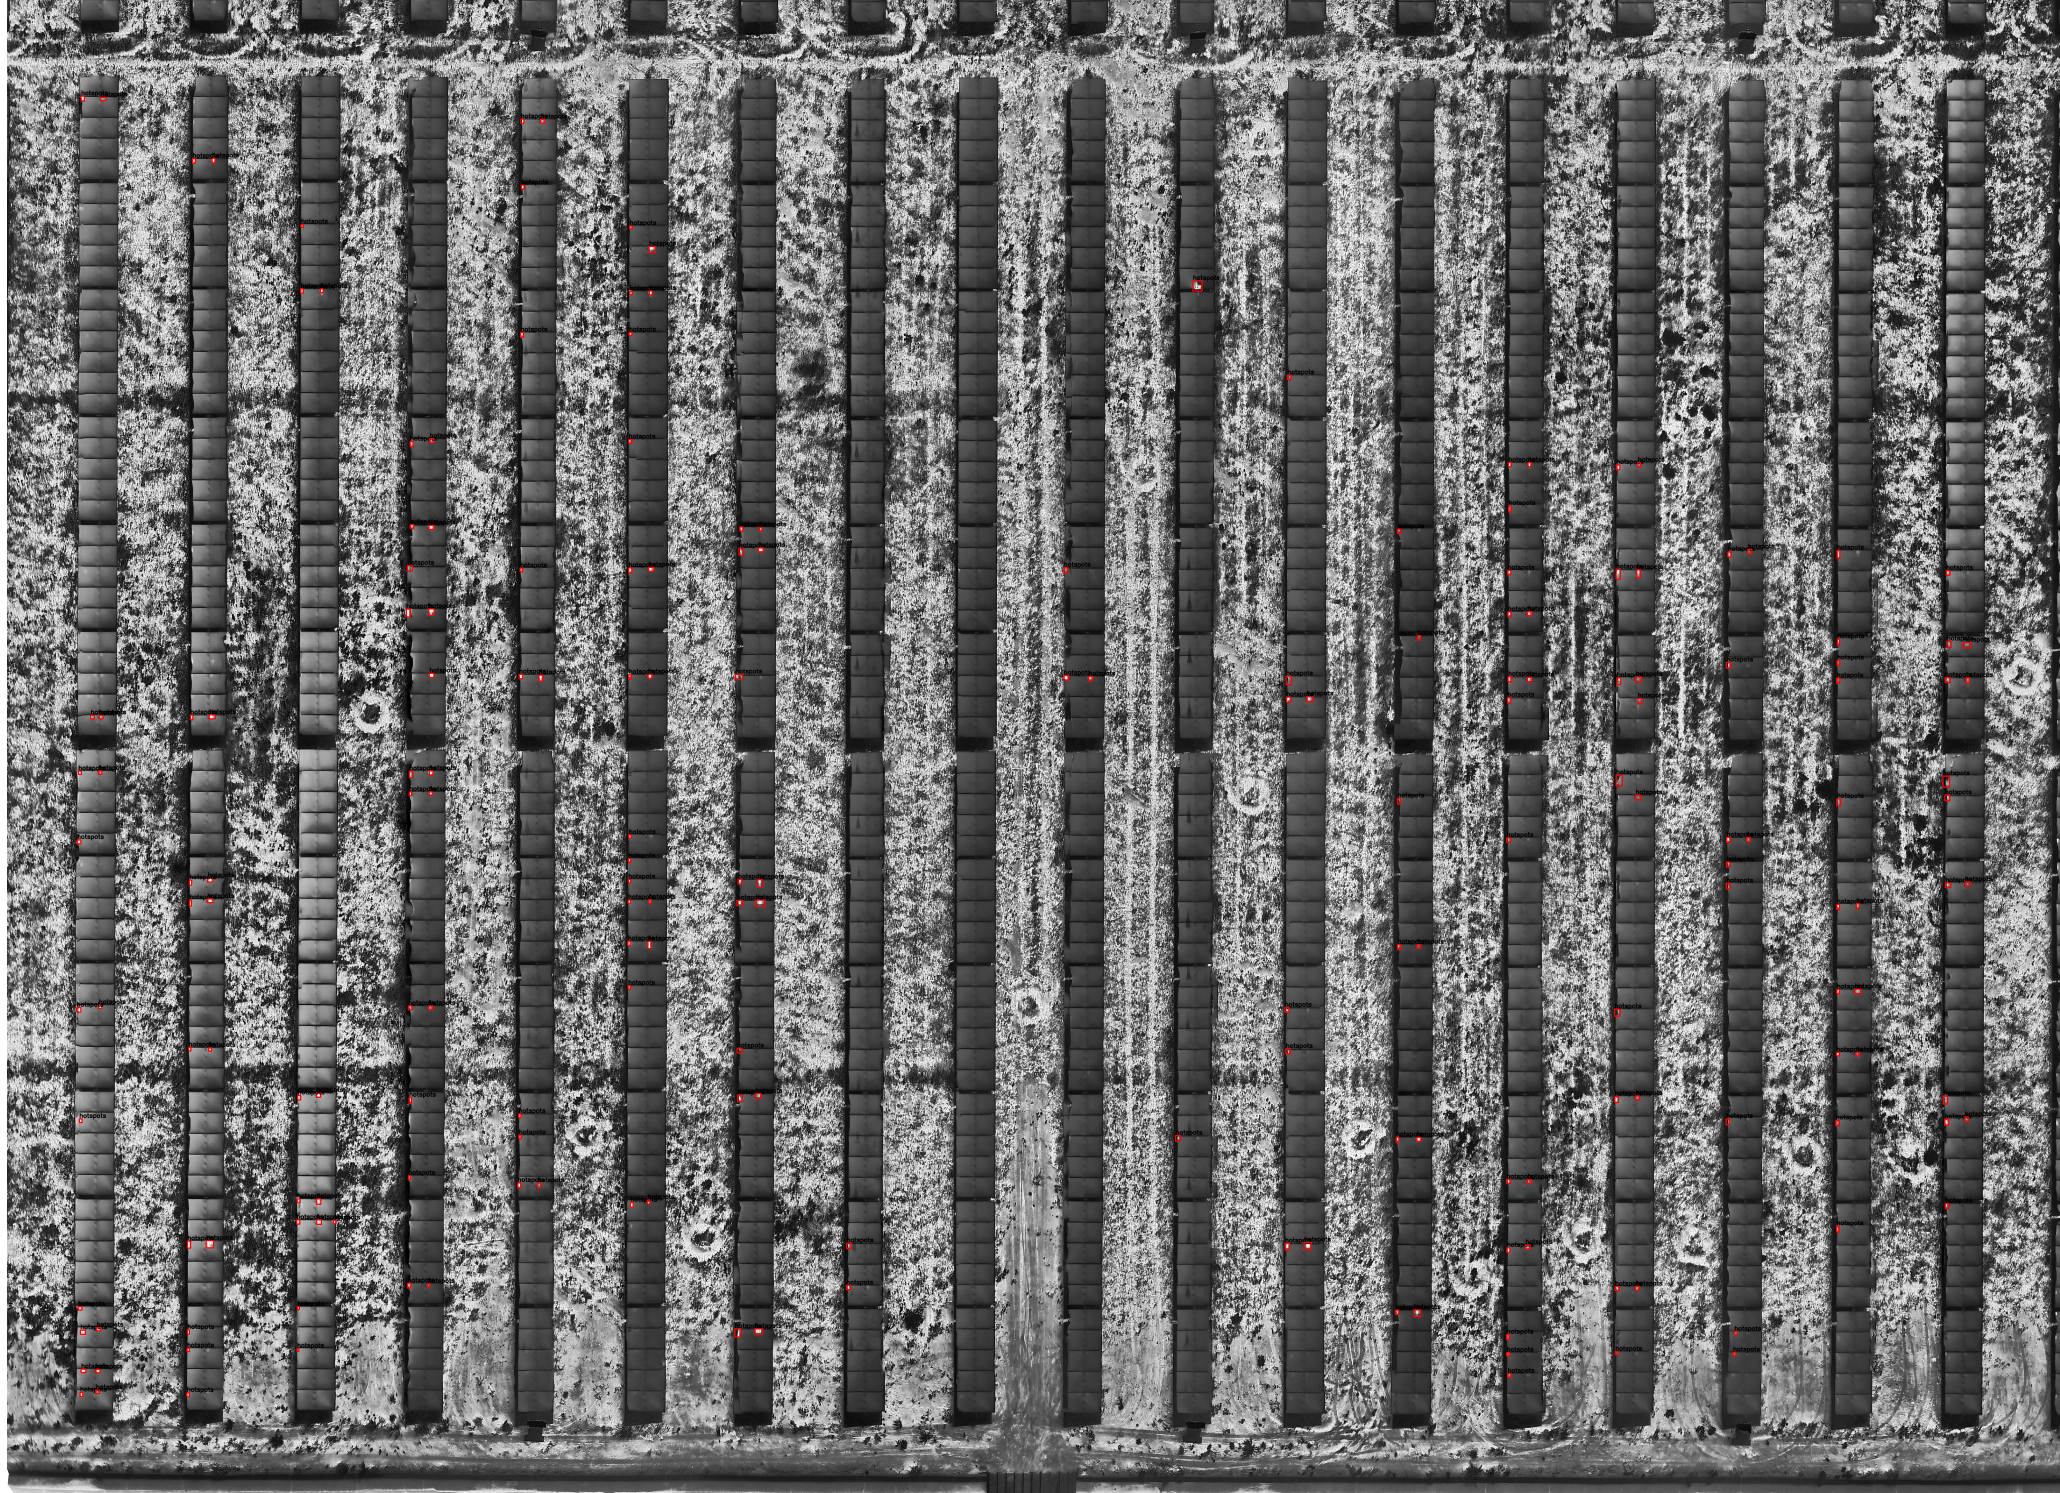
\includegraphics[width=0.8\textwidth]{report_images/ortho.png}%
\caption{Ortofoto}%
\end{figure}

%
\FloatBarrier%


\begin{figure}[h!]%
\centering%
\includegraphics[width=0.8\textwidth]{report_images/layer_img.pdf}%
\caption{Máscara dos Painéis}%
\end{figure}

%
\FloatBarrier%


\begin{table}[h!]%
\caption{Resumo dos Defeitos Identificados}%
\begin{tabular}{lll}%
\toprule%
Tipo de Problema&Local do Painel&Coordenadas\\%
\midrule%
Pontos Quentes (Hot Spots)&1{-}2&({-}40.54215518629289, {-}7.323360903612326)\\%
Pontos Quentes (Hot Spots)&1{-}2&({-}40.54215518629289, {-}7.323360903612326)\\%
Pontos Quentes (Hot Spots)&1{-}31&({-}40.5421564798669, {-}7.323712878967138)\\%
Pontos Quentes (Hot Spots)&1{-}31&({-}40.5421564798669, {-}7.323712878967138)\\%
Pontos Quentes (Hot Spots)&1{-}33&({-}40.54215676732779, {-}7.3237453821590766)\\%
Pontos Quentes (Hot Spots)&1{-}33&({-}40.54215676732779, {-}7.3237453821590766)\\%
Pontos Quentes (Hot Spots)&1{-}36&({-}40.54215676732779, {-}7.323779596045329)\\%
Pontos Quentes (Hot Spots)&1{-}44&({-}40.54215676732779, {-}7.323879243989036)\\%
Pontos Quentes (Hot Spots)&1{-}44&({-}40.54215676732779, {-}7.323879243989036)\\%
Pontos Quentes (Hot Spots)&1{-}49&({-}40.5421580609018, {-}7.323939831079272)\\%
Pontos Quentes (Hot Spots)&1{-}58&({-}40.5421580609018, {-}7.324050598536012)\\%
Pontos Quentes (Hot Spots)&1{-}59&({-}40.5421580609018, {-}7.324062003164762)\\%
Pontos Quentes (Hot Spots)&1{-}59&({-}40.5421580609018, {-}7.324062003164762)\\%
Pontos Quentes (Hot Spots)&1{-}61&({-}40.5421580609018, {-}7.324084812422263)\\%
Pontos Quentes (Hot Spots)&1{-}61&({-}40.5421580609018, {-}7.324084812422263)\\%
Pontos Quentes (Hot Spots)&1{-}62&({-}40.5421580609018, {-}7.3240962170510135)\\%
Pontos Quentes (Hot Spots)&1{-}62&({-}40.5421580609018, {-}7.3240962170510135)\\%
Pontos Quentes (Hot Spots)&2{-}5&({-}40.54208964520976, {-}7.323395117498578)\\%
Pontos Quentes (Hot Spots)&2{-}5&({-}40.54208964520976, {-}7.323395117498578)\\%
Pontos Quentes (Hot Spots)&2{-}31&({-}40.542092088627335, {-}7.323711881062122)\\%
Pontos Quentes (Hot Spots)&2{-}31&({-}40.542092088627335, {-}7.323711881062122)\\%
Pontos Quentes (Hot Spots)&2{-}38&({-}40.54209129810988, {-}7.323805684133595)\\%
Pontos Quentes (Hot Spots)&2{-}38&({-}40.54209129810988, {-}7.323805684133595)\\%
Pontos Quentes (Hot Spots)&2{-}39&({-}40.54209129810988, {-}7.323817088762346)\\%
Pontos Quentes (Hot Spots)&2{-}39&({-}40.54209129810988, {-}7.323817088762346)\\%
Pontos Quentes (Hot Spots)&2{-}46&({-}40.5420932384709, {-}7.323902053246536)\\%
Pontos Quentes (Hot Spots)&2{-}46&({-}40.5420932384709, {-}7.323902053246536)\\%
Pontos Quentes (Hot Spots)&2{-}55&({-}40.54209280727956, {-}7.324013105818994)\\%
Pontos Quentes (Hot Spots)&2{-}55&({-}40.54209280727956, {-}7.324013105818994)\\%
Pontos Quentes (Hot Spots)&2{-}59&({-}40.5420932384709, {-}7.324062003164762)\\%
Pontos Quentes (Hot Spots)&2{-}60&({-}40.5420932384709, {-}7.324073407793513)\\%
Pontos Quentes (Hot Spots)&2{-}62&({-}40.5420932384709, {-}7.3240962170510135)\\%
Pontos Quentes (Hot Spots)&3{-}8&({-}40.54202855977044, {-}7.323432610215595)\\%
Pontos Quentes (Hot Spots)&3{-}11&({-}40.54203014080534, {-}7.323470673164049)\\%
Pontos Quentes (Hot Spots)&3{-}11&({-}40.54203014080534, {-}7.323470673164049)\\%
\bottomrule%
\end{tabular}%
\end{table}

%
\FloatBarrier%


\begin{table}[h!]%
\caption{Resumo dos Defeitos Identificados (cont.)}%
\begin{tabular}{lll}%
\toprule%
Tipo de Problema&Local do Painel&Coordenadas\\%
\midrule%
Pontos Quentes (Hot Spots)&3{-}48&({-}40.54203042826623, {-}7.3239297094712565)\\%
Pontos Quentes (Hot Spots)&3{-}48&({-}40.54203042826623, {-}7.3239297094712565)\\%
Pontos Quentes (Hot Spots)&3{-}53&({-}40.54203014080534, {-}7.323990296561494)\\%
Pontos Quentes (Hot Spots)&3{-}53&({-}40.54203014080534, {-}7.323990296561494)\\%
Pontos Quentes (Hot Spots)&3{-}54&({-}40.54203014080534, {-}7.324001701190244)\\%
Pontos Quentes (Hot Spots)&3{-}54&({-}40.54203014080534, {-}7.324001701190244)\\%
Pontos Quentes (Hot Spots)&3{-}54&({-}40.54203014080534, {-}7.324001701190244)\\%
Pontos Quentes (Hot Spots)&3{-}58&({-}40.54203014080534, {-}7.324052166672465)\\%
Pontos Quentes (Hot Spots)&3{-}60&({-}40.54203014080534, {-}7.324074975929966)\\%
Pontos Quentes (Hot Spots)&4{-}18&({-}40.5419648871831, {-}7.323556920668975)\\%
Pontos Quentes (Hot Spots)&4{-}18&({-}40.5419648871831, {-}7.323556920668975)\\%
Pontos Quentes (Hot Spots)&4{-}22&({-}40.541966180757115, {-}7.323605247783306)\\%
Pontos Quentes (Hot Spots)&4{-}22&({-}40.541966180757115, {-}7.323605247783306)\\%
Pontos Quentes (Hot Spots)&4{-}24&({-}40.541966180757115, {-}7.323628057040806)\\%
Pontos Quentes (Hot Spots)&4{-}26&({-}40.541966180757115, {-}7.3236508662983075)\\%
Pontos Quentes (Hot Spots)&4{-}26&({-}40.541966180757115, {-}7.3236508662983075)\\%
Pontos Quentes (Hot Spots)&4{-}29&({-}40.54196689940934, {-}7.323689071804622)\\%
Pontos Quentes (Hot Spots)&4{-}33&({-}40.54196733060068, {-}7.3237453821590766)\\%
Pontos Quentes (Hot Spots)&4{-}33&({-}40.54196733060068, {-}7.3237453821590766)\\%
Pontos Quentes (Hot Spots)&4{-}34&({-}40.54196733060068, {-}7.323756786787827)\\%
Pontos Quentes (Hot Spots)&4{-}34&({-}40.54196733060068, {-}7.323756786787827)\\%
Pontos Quentes (Hot Spots)&4{-}44&({-}40.541965749565776, {-}7.323879243989036)\\%
Pontos Quentes (Hot Spots)&4{-}44&({-}40.541965749565776, {-}7.323879243989036)\\%
Pontos Quentes (Hot Spots)&4{-}48&({-}40.54196776179201, {-}7.32392899668196)\\%
Pontos Quentes (Hot Spots)&4{-}52&({-}40.54196776179201, {-}7.323974615196962)\\%
Pontos Quentes (Hot Spots)&4{-}57&({-}40.54196848044424, {-}7.324035915076496)\\%
Pontos Quentes (Hot Spots)&4{-}57&({-}40.54196848044424, {-}7.324035915076496)\\%
Pontos Quentes (Hot Spots)&5{-}3&({-}40.54190293936111, {-}7.323374161493248)\\%
Pontos Quentes (Hot Spots)&5{-}3&({-}40.54190293936111, {-}7.323374161493248)\\%
Pontos Quentes (Hot Spots)&5{-}6&({-}40.541900927134876, {-}7.323411654210266)\\%
Pontos Quentes (Hot Spots)&5{-}13&({-}40.54190063967398, {-}7.3234956207894415)\\%
Pontos Quentes (Hot Spots)&5{-}24&({-}40.54190293936111, {-}7.323628057040806)\\%
Pontos Quentes (Hot Spots)&5{-}29&({-}40.54190250816977, {-}7.323690925056793)\\%
Pontos Quentes (Hot Spots)&5{-}29&({-}40.54190250816977, {-}7.323690925056793)\\%
Pontos Quentes (Hot Spots)&5{-}49&({-}40.54190301122633, {-}7.323941114100007)\\%
\bottomrule%
\end{tabular}%
\end{table}

%
\FloatBarrier%


\begin{table}[h!]%
\caption{Resumo dos Defeitos Identificados (cont.)}%
\begin{tabular}{lll}%
\toprule%
Tipo de Problema&Local do Painel&Coordenadas\\%
\midrule%
Pontos Quentes (Hot Spots)&5{-}50&({-}40.54190301122633, {-}7.323952518728758)\\%
Pontos Quentes (Hot Spots)&5{-}52&({-}40.54190301122633, {-}7.3239753279862585)\\%
Pontos Quentes (Hot Spots)&5{-}52&({-}40.54190301122633, {-}7.3239753279862585)\\%
Pontos Quentes (Hot Spots)&6{-}8&({-}40.54183941050422, {-}7.323434463467767)\\%
Pontos Quentes (Hot Spots)&6{-}9&({-}40.54183941050422, {-}7.323445868096518)\\%
Pontos Quentes (Hot Spots)&6{-}11&({-}40.541839841695555, {-}7.32347281153194)\\%
Pontos Quentes (Hot Spots)&6{-}11&({-}40.541839841695555, {-}7.32347281153194)\\%
Pontos Quentes (Hot Spots)&6{-}13&({-}40.541839841695555, {-}7.3234956207894415)\\%
Pontos Quentes (Hot Spots)&6{-}18&({-}40.54184099153912, {-}7.323556920668975)\\%
Pontos Quentes (Hot Spots)&6{-}24&({-}40.54184142273046, {-}7.323628769830103)\\%
Pontos Quentes (Hot Spots)&6{-}24&({-}40.54184142273046, {-}7.323628769830103)\\%
Pontos Quentes (Hot Spots)&6{-}29&({-}40.54184012915644, {-}7.323690069709637)\\%
Pontos Quentes (Hot Spots)&6{-}29&({-}40.54184012915644, {-}7.323690069709637)\\%
Pontos Quentes (Hot Spots)&6{-}36&({-}40.54184012915644, {-}7.3237804513924845)\\%
Pontos Quentes (Hot Spots)&6{-}37&({-}40.54184099153912, {-}7.323795134852001)\\%
Pontos Quentes (Hot Spots)&6{-}38&({-}40.54184099153912, {-}7.323806539480751)\\%
Pontos Quentes (Hot Spots)&6{-}39&({-}40.54184099153912, {-}7.323817944109502)\\%
Pontos Quentes (Hot Spots)&6{-}39&({-}40.54184099153912, {-}7.323817944109502)\\%
Pontos Quentes (Hot Spots)&6{-}41&({-}40.54184099153912, {-}7.323840753367003)\\%
Pontos Quentes (Hot Spots)&6{-}41&({-}40.54184099153912, {-}7.323840753367003)\\%
Pontos Quentes (Hot Spots)&6{-}43&({-}40.54184099153912, {-}7.323867839360285)\\%
Pontos Quentes (Hot Spots)&6{-}53&({-}40.54184012915644, {-}7.323990296561494)\\%
Pontos Quentes (Hot Spots)&6{-}53&({-}40.54184012915644, {-}7.323990296561494)\\%
Pontos Quentes (Hot Spots)&7{-}22&({-}40.54177818133445, {-}7.323604820109727)\\%
Pontos Quentes (Hot Spots)&7{-}22&({-}40.54177818133445, {-}7.323604820109727)\\%
Pontos Quentes (Hot Spots)&7{-}23&({-}40.54177818133445, {-}7.323616224738478)\\%
Pontos Quentes (Hot Spots)&7{-}23&({-}40.54177818133445, {-}7.323616224738478)\\%
Pontos Quentes (Hot Spots)&7{-}29&({-}40.54177818133445, {-}7.323690925056793)\\%
Pontos Quentes (Hot Spots)&7{-}38&({-}40.54177861252579, {-}7.3238088204065015)\\%
Pontos Quentes (Hot Spots)&7{-}38&({-}40.54177861252579, {-}7.3238088204065015)\\%
Pontos Quentes (Hot Spots)&7{-}39&({-}40.54177861252579, {-}7.323820225035252)\\%
Pontos Quentes (Hot Spots)&7{-}39&({-}40.54177861252579, {-}7.323820225035252)\\%
Pontos Quentes (Hot Spots)&7{-}46&({-}40.541775881647325, {-}7.323902480920115)\\%
Pontos Quentes (Hot Spots)&7{-}48&({-}40.54177775014311, {-}7.323930279702694)\\%
Pontos Quentes (Hot Spots)&7{-}48&({-}40.54177775014311, {-}7.323930279702694)\\%
\bottomrule%
\end{tabular}%
\end{table}

%
\FloatBarrier%


\begin{table}[h!]%
\caption{Resumo dos Defeitos Identificados (cont.)}%
\begin{tabular}{lll}%
\toprule%
Tipo de Problema&Local do Painel&Coordenadas\\%
\midrule%
Pontos Quentes (Hot Spots)&7{-}59&({-}40.54177775014311, {-}7.324063571301215)\\%
Pontos Quentes (Hot Spots)&7{-}59&({-}40.54177775014311, {-}7.324063571301215)\\%
Pontos Quentes (Hot Spots)&8{-}55&({-}40.5417150836689, {-}7.324013818608291)\\%
Pontos Quentes (Hot Spots)&8{-}57&({-}40.5417150836689, {-}7.324036627865793)\\%
Pontos Quentes (Hot Spots)&10{-}24&({-}40.54158860087689, {-}7.323628769830103)\\%
Pontos Quentes (Hot Spots)&10{-}29&({-}40.54158946325956, {-}7.323690925056793)\\%
Pontos Quentes (Hot Spots)&10{-}29&({-}40.54158946325956, {-}7.323690925056793)\\%
Pontos Quentes (Hot Spots)&11{-}10&({-}40.541522916063315, {-}7.323457272725268)\\%
Pontos Quentes (Hot Spots)&11{-}50&({-}40.54152507202, {-}7.323953088960195)\\%
Pontos Quentes (Hot Spots)&12{-}15&({-}40.541460968241324, {-}7.323518430046942)\\%
Pontos Quentes (Hot Spots)&12{-}29&({-}40.54146125570222, {-}7.323691352730371)\\%
Pontos Quentes (Hot Spots)&12{-}30&({-}40.54146125570222, {-}7.323702757359122)\\%
Pontos Quentes (Hot Spots)&12{-}30&({-}40.54146125570222, {-}7.323702757359122)\\%
Pontos Quentes (Hot Spots)&12{-}44&({-}40.54146211808489, {-}7.32388052700977)\\%
Pontos Quentes (Hot Spots)&12{-}46&({-}40.54146211808489, {-}7.323903336267271)\\%
Pontos Quentes (Hot Spots)&12{-}55&({-}40.54146283673712, {-}7.324013818608291)\\%
Pontos Quentes (Hot Spots)&12{-}55&({-}40.54146283673712, {-}7.324013818608291)\\%
Pontos Quentes (Hot Spots)&13{-}22&({-}40.541398589227995, {-}7.323607671266915)\\%
Pontos Quentes (Hot Spots)&13{-}27&({-}40.54139801430621, {-}7.323668543472871)\\%
Pontos Quentes (Hot Spots)&13{-}34&({-}40.54139815803666, {-}7.323758640039999)\\%
Pontos Quentes (Hot Spots)&13{-}41&({-}40.54139729565399, {-}7.32384374708205)\\%
Pontos Quentes (Hot Spots)&13{-}41&({-}40.54139729565399, {-}7.32384374708205)\\%
Pontos Quentes (Hot Spots)&13{-}50&({-}40.54139873295844, {-}7.323954371980929)\\%
Pontos Quentes (Hot Spots)&13{-}50&({-}40.54139873295844, {-}7.323954371980929)\\%
Pontos Quentes (Hot Spots)&13{-}58&({-}40.54139973907156, {-}7.3240533071353395)\\%
Pontos Quentes (Hot Spots)&13{-}58&({-}40.54139973907156, {-}7.3240533071353395)\\%
Pontos Quentes (Hot Spots)&14{-}19&({-}40.541335347831996, {-}7.323569750876319)\\%
Pontos Quentes (Hot Spots)&14{-}19&({-}40.541335347831996, {-}7.323569750876319)\\%
Pontos Quentes (Hot Spots)&14{-}21&({-}40.541335347831996, {-}7.323592560133821)\\%
Pontos Quentes (Hot Spots)&14{-}24&({-}40.54133520410155, {-}7.323631478429432)\\%
Pontos Quentes (Hot Spots)&14{-}26&({-}40.54133520410155, {-}7.323654287686932)\\%
Pontos Quentes (Hot Spots)&14{-}26&({-}40.54133520410155, {-}7.323654287686932)\\%
Pontos Quentes (Hot Spots)&14{-}29&({-}40.541335060371104, {-}7.323690925056793)\\%
Pontos Quentes (Hot Spots)&14{-}29&({-}40.541335060371104, {-}7.323690925056793)\\%
Pontos Quentes (Hot Spots)&14{-}30&({-}40.541335060371104, {-}7.323702329685544)\\%
\bottomrule%
\end{tabular}%
\end{table}

%
\FloatBarrier%


\begin{table}[h!]%
\caption{Resumo dos Defeitos Identificados (cont.)}%
\begin{tabular}{lll}%
\toprule%
Tipo de Problema&Local do Painel&Coordenadas\\%
\midrule%
Pontos Quentes (Hot Spots)&14{-}36&({-}40.54133477291021, {-}7.323781876971078)\\%
Pontos Quentes (Hot Spots)&14{-}52&({-}40.54133491664066, {-}7.323977181238431)\\%
Pontos Quentes (Hot Spots)&14{-}52&({-}40.54133491664066, {-}7.323977181238431)\\%
Pontos Quentes (Hot Spots)&14{-}55&({-}40.541334629179765, {-}7.324015244186885)\\%
Pontos Quentes (Hot Spots)&14{-}55&({-}40.541334629179765, {-}7.324015244186885)\\%
Pontos Quentes (Hot Spots)&14{-}59&({-}40.54133477291021, {-}7.324065424553387)\\%
Pontos Quentes (Hot Spots)&14{-}60&({-}40.54133477291021, {-}7.324076829182138)\\%
Pontos Quentes (Hot Spots)&14{-}61&({-}40.54133477291021, {-}7.324088233810889)\\%
Pontos Quentes (Hot Spots)&15{-}19&({-}40.541271100322874, {-}7.323569180644882)\\%
Pontos Quentes (Hot Spots)&15{-}19&({-}40.541271100322874, {-}7.323569180644882)\\%
Pontos Quentes (Hot Spots)&15{-}24&({-}40.541271818975105, {-}7.3236304805244155)\\%
Pontos Quentes (Hot Spots)&15{-}24&({-}40.541271818975105, {-}7.3236304805244155)\\%
Pontos Quentes (Hot Spots)&15{-}29&({-}40.541271100322874, {-}7.323692350635387)\\%
Pontos Quentes (Hot Spots)&15{-}29&({-}40.541271100322874, {-}7.323692350635387)\\%
Pontos Quentes (Hot Spots)&15{-}30&({-}40.541271100322874, {-}7.3237037552641375)\\%
Pontos Quentes (Hot Spots)&15{-}33&({-}40.54127153151421, {-}7.323747663084827)\\%
Pontos Quentes (Hot Spots)&15{-}34&({-}40.54127153151421, {-}7.323759067713578)\\%
Pontos Quentes (Hot Spots)&15{-}44&({-}40.541272250166436, {-}7.323881239799067)\\%
Pontos Quentes (Hot Spots)&15{-}48&({-}40.54127325627955, {-}7.323930992491991)\\%
Pontos Quentes (Hot Spots)&15{-}48&({-}40.54127325627955, {-}7.323930992491991)\\%
Pontos Quentes (Hot Spots)&15{-}57&({-}40.541271387783766, {-}7.3240380534443865)\\%
Pontos Quentes (Hot Spots)&15{-}57&({-}40.541271387783766, {-}7.3240380534443865)\\%
Pontos Quentes (Hot Spots)&15{-}60&({-}40.541272250166436, {-}7.324076829182138)\\%
Pontos Quentes (Hot Spots)&16{-}23&({-}40.54120771519643, {-}7.323619503569243)\\%
Pontos Quentes (Hot Spots)&16{-}23&({-}40.54120771519643, {-}7.323619503569243)\\%
Pontos Quentes (Hot Spots)&16{-}28&({-}40.541207427735536, {-}7.323680946006637)\\%
Pontos Quentes (Hot Spots)&16{-}36&({-}40.54120800265732, {-}7.3237814492975)\\%
Pontos Quentes (Hot Spots)&16{-}36&({-}40.54120800265732, {-}7.3237814492975)\\%
Pontos Quentes (Hot Spots)&16{-}37&({-}40.541208721309545, {-}7.323797415777751)\\%
Pontos Quentes (Hot Spots)&16{-}38&({-}40.541208721309545, {-}7.3238088204065015)\\%
Pontos Quentes (Hot Spots)&16{-}49&({-}40.54120843384865, {-}7.323942967352179)\\%
Pontos Quentes (Hot Spots)&16{-}59&({-}40.54120972742266, {-}7.324065424553387)\\%
Pontos Quentes (Hot Spots)&16{-}60&({-}40.54120972742266, {-}7.324076829182138)\\%
Pontos Quentes (Hot Spots)&17{-}23&({-}40.54114447380042, {-}7.323619503569243)\\%
Pontos Quentes (Hot Spots)&17{-}27&({-}40.5411453361831, {-}7.323669541377886)\\%
\bottomrule%
\end{tabular}%
\end{table}

%
\FloatBarrier%


\begin{table}[h!]%
\caption{Resumo dos Defeitos Identificados (cont.)}%
\begin{tabular}{lll}%
\toprule%
Tipo de Problema&Local do Painel&Coordenadas\\%
\midrule%
Pontos Quentes (Hot Spots)&17{-}28&({-}40.5411453361831, {-}7.323680946006637)\\%
Pontos Quentes (Hot Spots)&17{-}29&({-}40.5411453361831, {-}7.323692350635387)\\%
Pontos Quentes (Hot Spots)&17{-}34&({-}40.54114483312654, {-}7.323759637945015)\\%
Pontos Quentes (Hot Spots)&17{-}39&({-}40.541145479913546, {-}7.323820937824549)\\%
Pontos Quentes (Hot Spots)&17{-}39&({-}40.541145479913546, {-}7.323820937824549)\\%
Pontos Quentes (Hot Spots)&17{-}43&({-}40.541144761261314, {-}7.323870405401754)\\%
Pontos Quentes (Hot Spots)&17{-}43&({-}40.541144761261314, {-}7.323870405401754)\\%
Pontos Quentes (Hot Spots)&17{-}46&({-}40.541144761261314, {-}7.3239046192880055)\\%
Pontos Quentes (Hot Spots)&17{-}46&({-}40.541144761261314, {-}7.3239046192880055)\\%
Pontos Quentes (Hot Spots)&17{-}49&({-}40.54114468939609, {-}7.323942967352179)\\%
Pontos Quentes (Hot Spots)&17{-}54&({-}40.54114504872221, {-}7.324004694905291)\\%
Pontos Quentes (Hot Spots)&18{-}24&({-}40.54108209478709, {-}7.323631478429432)\\%
Pontos Quentes (Hot Spots)&18{-}27&({-}40.54108209478709, {-}7.323669541377886)\\%
Pontos Quentes (Hot Spots)&18{-}27&({-}40.54108209478709, {-}7.323669541377886)\\%
Pontos Quentes (Hot Spots)&18{-}29&({-}40.54108209478709, {-}7.323692350635387)\\%
Pontos Quentes (Hot Spots)&18{-}29&({-}40.54108209478709, {-}7.323692350635387)\\%
Pontos Quentes (Hot Spots)&18{-}33&({-}40.54108338836111, {-}7.323747663084827)\\%
Pontos Quentes (Hot Spots)&18{-}34&({-}40.54108338836111, {-}7.323759067713578)\\%
Pontos Quentes (Hot Spots)&18{-}38&({-}40.54108295716977, {-}7.323809533195798)\\%
Pontos Quentes (Hot Spots)&18{-}38&({-}40.54108295716977, {-}7.323809533195798)\\%
Pontos Quentes (Hot Spots)&18{-}48&({-}40.541084394474225, {-}7.323930992491991)\\%
Pontos Quentes (Hot Spots)&18{-}49&({-}40.541084394474225, {-}7.323942397120741)\\%
Pontos Quentes (Hot Spots)&18{-}49&({-}40.541084394474225, {-}7.323942397120741)\\%
Pontos Quentes (Hot Spots)&18{-}53&({-}40.54108353209155, {-}7.323992434929385)\\%
\bottomrule%
\end{tabular}%
\end{table}

%
\FloatBarrier%
\newpage%
\section{Pontos Quentes (Hot Spots)}%
Foram detectados pontos quentes nas placas abaixo.\newline%
%
\subsubsection{Painel 1-2}%


\begin{figure}[h!]%
\centering%
\subfloat[Recorte do Painel em Análise]{\includegraphics[width=0.31\linewidth]{report_images/hotspots_(1-2)_layer.pdf}}%
\hfill%
\subfloat[Localização do Problema]{\includegraphics[width=0.31\linewidth]{report_images/hotspots_(1-2)_cropped.jpg}}%
\hfill%
\subfloat[Imagem Original do Drone]{\includegraphics[width=0.31\linewidth]{report_images/hotspots_(1-2).jpg}}%
\caption{Imagens do Painel n. 2 da coluna n. 1.}%
\end{figure}

%
\FloatBarrier%
No painel 1{-}2, há sinais de pontos quentes conforme as figuras acima.\newline%
%
\subsubsection{Painel 1-31}%


\begin{figure}[h!]%
\centering%
\subfloat[Recorte do Painel em Análise]{\includegraphics[width=0.31\linewidth]{report_images/hotspots_(1-31)_layer.pdf}}%
\hfill%
\subfloat[Localização do Problema]{\includegraphics[width=0.31\linewidth]{report_images/hotspots_(1-31)_cropped.jpg}}%
\hfill%
\subfloat[Imagem Original do Drone]{\includegraphics[width=0.31\linewidth]{report_images/hotspots_(1-31).jpg}}%
\caption{Imagens do Painel n. 31 da coluna n. 1.}%
\end{figure}

%
\FloatBarrier%
No painel 1{-}31, há sinais de pontos quentes conforme as figuras acima.\newline%
%
\subsubsection{Painel 1-33}%


\begin{figure}[h!]%
\centering%
\subfloat[Recorte do Painel em Análise]{\includegraphics[width=0.31\linewidth]{report_images/hotspots_(1-33)_layer.pdf}}%
\hfill%
\subfloat[Localização do Problema]{\includegraphics[width=0.31\linewidth]{report_images/hotspots_(1-33)_cropped.jpg}}%
\hfill%
\subfloat[Imagem Original do Drone]{\includegraphics[width=0.31\linewidth]{report_images/hotspots_(1-33).jpg}}%
\caption{Imagens do Painel n. 33 da coluna n. 1.}%
\end{figure}

%
\FloatBarrier%
No painel 1{-}33, há sinais de pontos quentes conforme as figuras acima.\newline%
%
\subsubsection{Painel 1-36}%


\begin{figure}[h!]%
\centering%
\subfloat[Recorte do Painel em Análise]{\includegraphics[width=0.31\linewidth]{report_images/hotspots_(1-36)_layer.pdf}}%
\hfill%
\subfloat[Localização do Problema]{\includegraphics[width=0.31\linewidth]{report_images/hotspots_(1-36)_cropped.jpg}}%
\hfill%
\subfloat[Imagem Original do Drone]{\includegraphics[width=0.31\linewidth]{report_images/hotspots_(1-36).jpg}}%
\caption{Imagens do Painel n. 36 da coluna n. 1.}%
\end{figure}

%
\FloatBarrier%
No painel 1{-}36, há sinais de pontos quentes conforme as figuras acima.\newline%
%
\subsubsection{Painel 1-44}%


\begin{figure}[h!]%
\centering%
\subfloat[Recorte do Painel em Análise]{\includegraphics[width=0.31\linewidth]{report_images/hotspots_(1-44)_layer.pdf}}%
\hfill%
\subfloat[Localização do Problema]{\includegraphics[width=0.31\linewidth]{report_images/hotspots_(1-44)_cropped.jpg}}%
\hfill%
\subfloat[Imagem Original do Drone]{\includegraphics[width=0.31\linewidth]{report_images/hotspots_(1-44).jpg}}%
\caption{Imagens do Painel n. 44 da coluna n. 1.}%
\end{figure}

%
\FloatBarrier%
No painel 1{-}44, há sinais de pontos quentes conforme as figuras acima.\newline%
%
\subsubsection{Painel 1-49}%


\begin{figure}[h!]%
\centering%
\subfloat[Recorte do Painel em Análise]{\includegraphics[width=0.31\linewidth]{report_images/hotspots_(1-49)_layer.pdf}}%
\hfill%
\subfloat[Localização do Problema]{\includegraphics[width=0.31\linewidth]{report_images/hotspots_(1-49)_cropped.jpg}}%
\hfill%
\subfloat[Imagem Original do Drone]{\includegraphics[width=0.31\linewidth]{report_images/hotspots_(1-49).jpg}}%
\caption{Imagens do Painel n. 49 da coluna n. 1.}%
\end{figure}

%
\FloatBarrier%
No painel 1{-}49, há sinais de pontos quentes conforme as figuras acima.\newline%
%
\subsubsection{Painel 1-58}%


\begin{figure}[h!]%
\centering%
\subfloat[Recorte do Painel em Análise]{\includegraphics[width=0.31\linewidth]{report_images/hotspots_(1-58)_layer.pdf}}%
\hfill%
\subfloat[Localização do Problema]{\includegraphics[width=0.31\linewidth]{report_images/hotspots_(1-58)_cropped.jpg}}%
\hfill%
\subfloat[Imagem Original do Drone]{\includegraphics[width=0.31\linewidth]{report_images/hotspots_(1-58).jpg}}%
\caption{Imagens do Painel n. 58 da coluna n. 1.}%
\end{figure}

%
\FloatBarrier%
No painel 1{-}58, há sinais de pontos quentes conforme as figuras acima.\newline%
%
\subsubsection{Painel 1-59}%


\begin{figure}[h!]%
\centering%
\subfloat[Recorte do Painel em Análise]{\includegraphics[width=0.31\linewidth]{report_images/hotspots_(1-59)_layer.pdf}}%
\hfill%
\subfloat[Localização do Problema]{\includegraphics[width=0.31\linewidth]{report_images/hotspots_(1-59)_cropped.jpg}}%
\hfill%
\subfloat[Imagem Original do Drone]{\includegraphics[width=0.31\linewidth]{report_images/hotspots_(1-59).jpg}}%
\caption{Imagens do Painel n. 59 da coluna n. 1.}%
\end{figure}

%
\FloatBarrier%
No painel 1{-}59, há sinais de pontos quentes conforme as figuras acima.\newline%
%
\subsubsection{Painel 1-61}%


\begin{figure}[h!]%
\centering%
\subfloat[Recorte do Painel em Análise]{\includegraphics[width=0.31\linewidth]{report_images/hotspots_(1-61)_layer.pdf}}%
\hfill%
\subfloat[Localização do Problema]{\includegraphics[width=0.31\linewidth]{report_images/hotspots_(1-61)_cropped.jpg}}%
\hfill%
\subfloat[Imagem Original do Drone]{\includegraphics[width=0.31\linewidth]{report_images/hotspots_(1-61).jpg}}%
\caption{Imagens do Painel n. 61 da coluna n. 1.}%
\end{figure}

%
\FloatBarrier%
No painel 1{-}61, há sinais de pontos quentes conforme as figuras acima.\newline%
%
\subsubsection{Painel 1-62}%


\begin{figure}[h!]%
\centering%
\subfloat[Recorte do Painel em Análise]{\includegraphics[width=0.31\linewidth]{report_images/hotspots_(1-62)_layer.pdf}}%
\hfill%
\subfloat[Localização do Problema]{\includegraphics[width=0.31\linewidth]{report_images/hotspots_(1-62)_cropped.jpg}}%
\hfill%
\subfloat[Imagem Original do Drone]{\includegraphics[width=0.31\linewidth]{report_images/hotspots_(1-62).jpg}}%
\caption{Imagens do Painel n. 62 da coluna n. 1.}%
\end{figure}

%
\FloatBarrier%
No painel 1{-}62, há sinais de pontos quentes conforme as figuras acima.\newline%
%
\subsubsection{Painel 2-5}%


\begin{figure}[h!]%
\centering%
\subfloat[Recorte do Painel em Análise]{\includegraphics[width=0.31\linewidth]{report_images/hotspots_(2-5)_layer.pdf}}%
\hfill%
\subfloat[Localização do Problema]{\includegraphics[width=0.31\linewidth]{report_images/hotspots_(2-5)_cropped.jpg}}%
\hfill%
\subfloat[Imagem Original do Drone]{\includegraphics[width=0.31\linewidth]{report_images/hotspots_(2-5).jpg}}%
\caption{Imagens do Painel n. 5 da coluna n. 2.}%
\end{figure}

%
\FloatBarrier%
No painel 2{-}5, há sinais de pontos quentes conforme as figuras acima.\newline%
%
\subsubsection{Painel 2-31}%


\begin{figure}[h!]%
\centering%
\subfloat[Recorte do Painel em Análise]{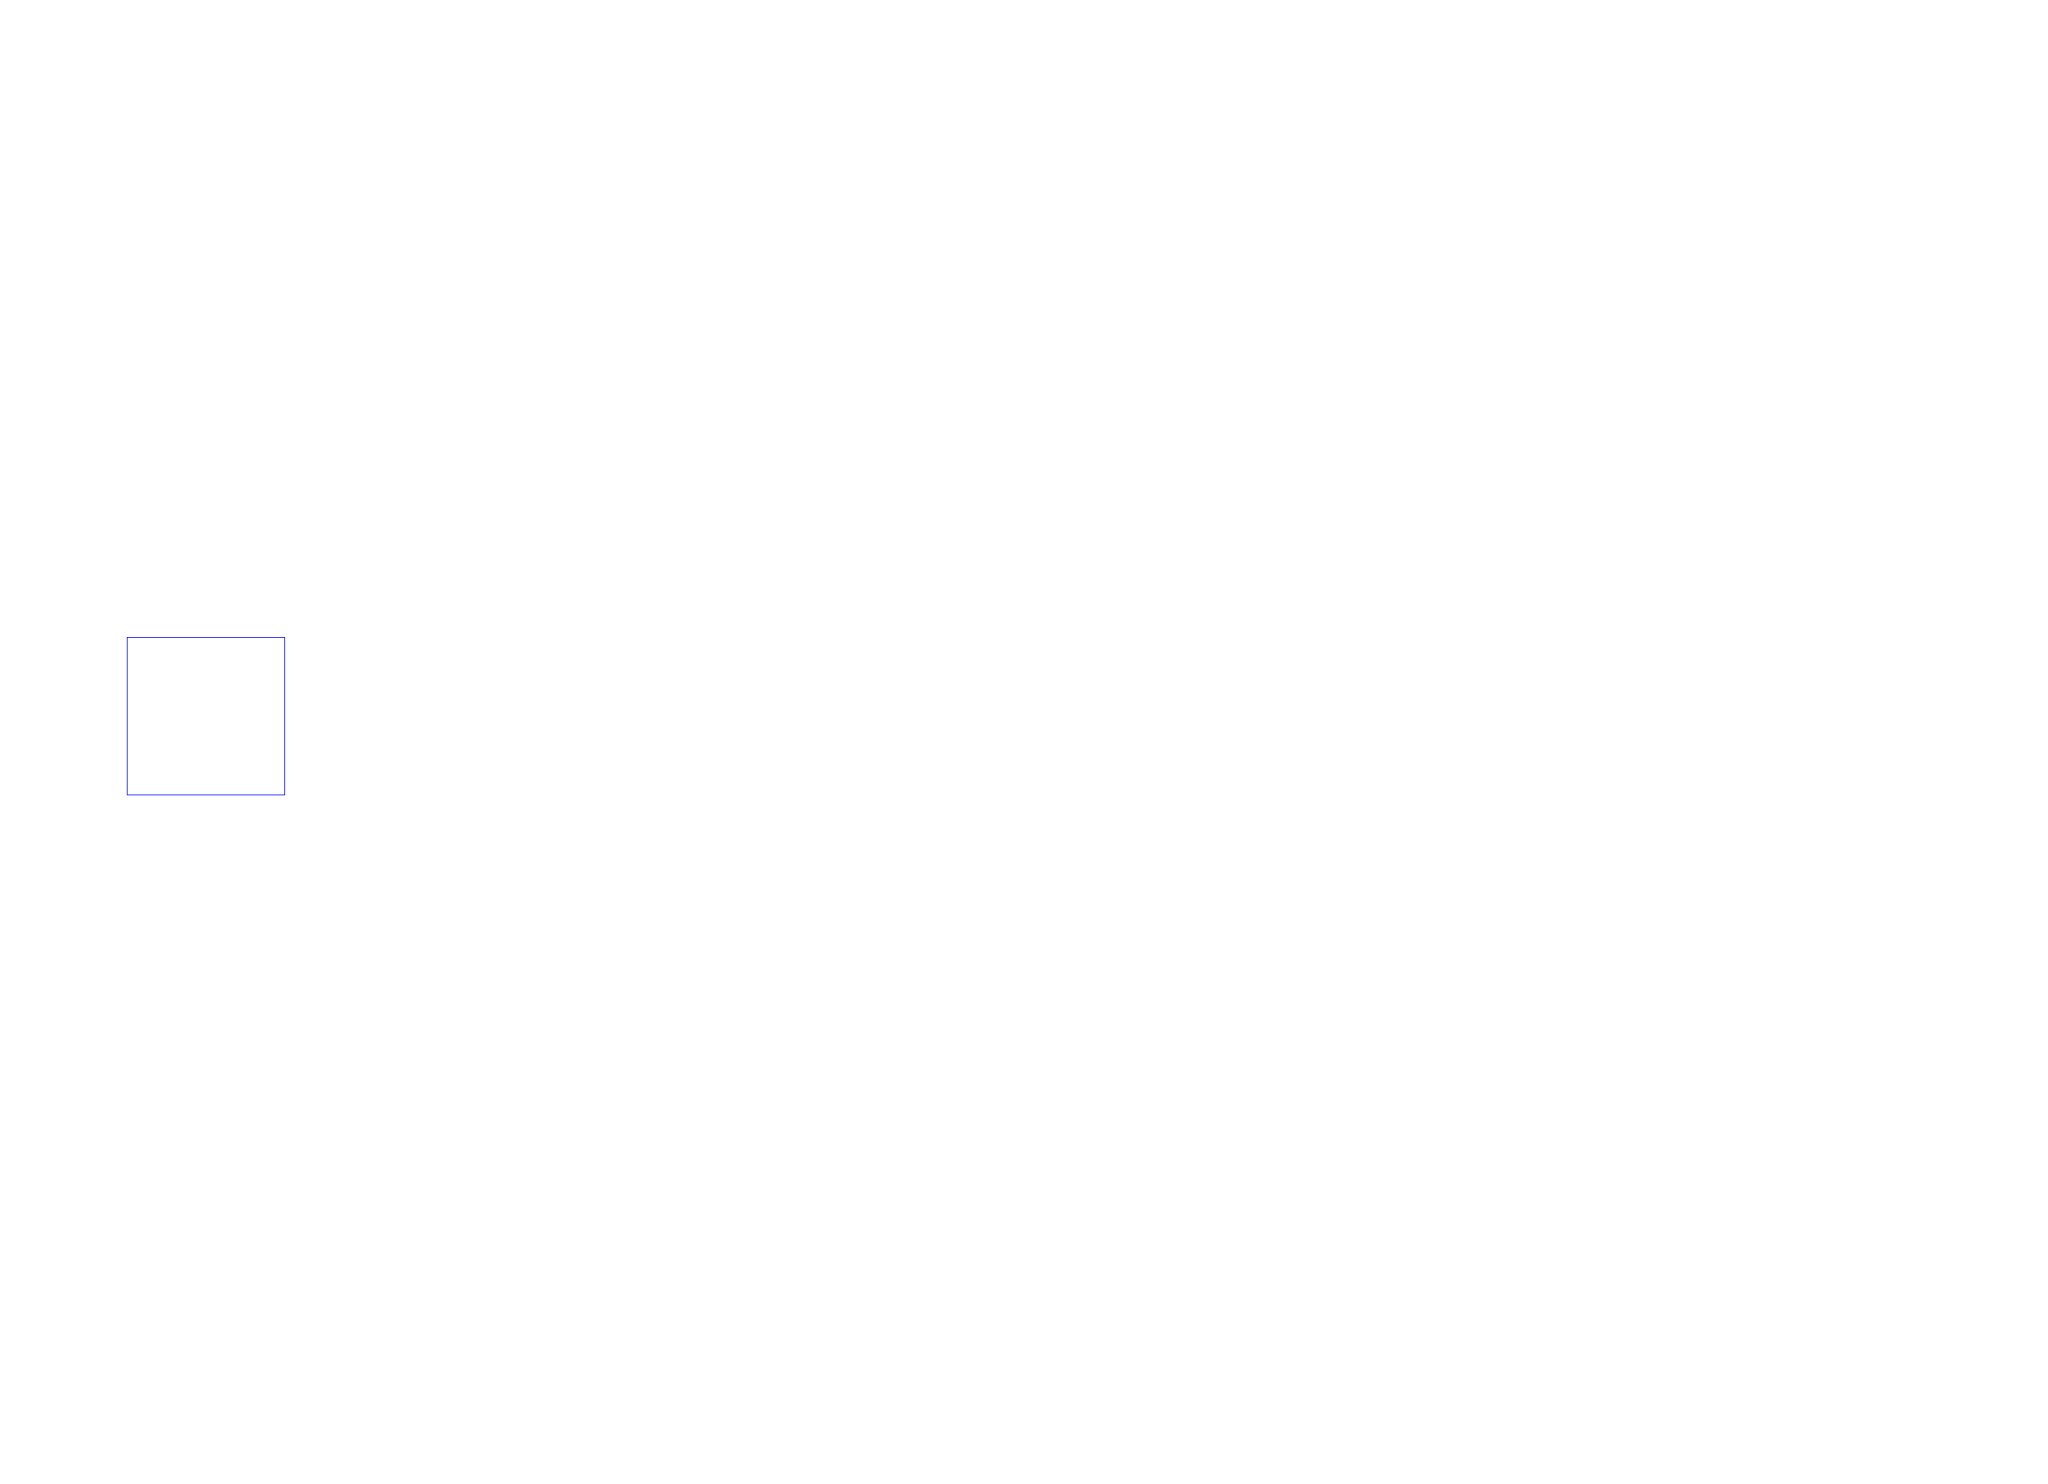
\includegraphics[width=0.31\linewidth]{report_images/hotspots_(2-31)_layer.pdf}}%
\hfill%
\subfloat[Localização do Problema]{\includegraphics[width=0.31\linewidth]{report_images/hotspots_(2-31)_cropped.jpg}}%
\hfill%
\subfloat[Imagem Original do Drone]{\includegraphics[width=0.31\linewidth]{report_images/hotspots_(2-31).jpg}}%
\caption{Imagens do Painel n. 31 da coluna n. 2.}%
\end{figure}

%
\FloatBarrier%
No painel 2{-}31, há sinais de pontos quentes conforme as figuras acima.\newline%
%
\subsubsection{Painel 2-38}%


\begin{figure}[h!]%
\centering%
\subfloat[Recorte do Painel em Análise]{\includegraphics[width=0.31\linewidth]{report_images/hotspots_(2-38)_layer.pdf}}%
\hfill%
\subfloat[Localização do Problema]{\includegraphics[width=0.31\linewidth]{report_images/hotspots_(2-38)_cropped.jpg}}%
\hfill%
\subfloat[Imagem Original do Drone]{\includegraphics[width=0.31\linewidth]{report_images/hotspots_(2-38).jpg}}%
\caption{Imagens do Painel n. 38 da coluna n. 2.}%
\end{figure}

%
\FloatBarrier%
No painel 2{-}38, há sinais de pontos quentes conforme as figuras acima.\newline%
%
\subsubsection{Painel 2-39}%


\begin{figure}[h!]%
\centering%
\subfloat[Recorte do Painel em Análise]{\includegraphics[width=0.31\linewidth]{report_images/hotspots_(2-39)_layer.pdf}}%
\hfill%
\subfloat[Localização do Problema]{\includegraphics[width=0.31\linewidth]{report_images/hotspots_(2-39)_cropped.jpg}}%
\hfill%
\subfloat[Imagem Original do Drone]{\includegraphics[width=0.31\linewidth]{report_images/hotspots_(2-39).jpg}}%
\caption{Imagens do Painel n. 39 da coluna n. 2.}%
\end{figure}

%
\FloatBarrier%
No painel 2{-}39, há sinais de pontos quentes conforme as figuras acima.\newline%
%
\subsubsection{Painel 2-46}%


\begin{figure}[h!]%
\centering%
\subfloat[Recorte do Painel em Análise]{\includegraphics[width=0.31\linewidth]{report_images/hotspots_(2-46)_layer.pdf}}%
\hfill%
\subfloat[Localização do Problema]{\includegraphics[width=0.31\linewidth]{report_images/hotspots_(2-46)_cropped.jpg}}%
\hfill%
\subfloat[Imagem Original do Drone]{\includegraphics[width=0.31\linewidth]{report_images/hotspots_(2-46).jpg}}%
\caption{Imagens do Painel n. 46 da coluna n. 2.}%
\end{figure}

%
\FloatBarrier%
No painel 2{-}46, há sinais de pontos quentes conforme as figuras acima.\newline%
%
\subsubsection{Painel 2-55}%


\begin{figure}[h!]%
\centering%
\subfloat[Recorte do Painel em Análise]{\includegraphics[width=0.31\linewidth]{report_images/hotspots_(2-55)_layer.pdf}}%
\hfill%
\subfloat[Localização do Problema]{\includegraphics[width=0.31\linewidth]{report_images/hotspots_(2-55)_cropped.jpg}}%
\hfill%
\subfloat[Imagem Original do Drone]{\includegraphics[width=0.31\linewidth]{report_images/hotspots_(2-55).jpg}}%
\caption{Imagens do Painel n. 55 da coluna n. 2.}%
\end{figure}

%
\FloatBarrier%
No painel 2{-}55, há sinais de pontos quentes conforme as figuras acima.\newline%
%
\subsubsection{Painel 2-59}%


\begin{figure}[h!]%
\centering%
\subfloat[Recorte do Painel em Análise]{\includegraphics[width=0.31\linewidth]{report_images/hotspots_(2-59)_layer.pdf}}%
\hfill%
\subfloat[Localização do Problema]{\includegraphics[width=0.31\linewidth]{report_images/hotspots_(2-59)_cropped.jpg}}%
\hfill%
\subfloat[Imagem Original do Drone]{\includegraphics[width=0.31\linewidth]{report_images/hotspots_(2-59).jpg}}%
\caption{Imagens do Painel n. 59 da coluna n. 2.}%
\end{figure}

%
\FloatBarrier%
No painel 2{-}59, há sinais de pontos quentes conforme as figuras acima.\newline%
%
\subsubsection{Painel 2-60}%


\begin{figure}[h!]%
\centering%
\subfloat[Recorte do Painel em Análise]{\includegraphics[width=0.31\linewidth]{report_images/hotspots_(2-60)_layer.pdf}}%
\hfill%
\subfloat[Localização do Problema]{\includegraphics[width=0.31\linewidth]{report_images/hotspots_(2-60)_cropped.jpg}}%
\hfill%
\subfloat[Imagem Original do Drone]{\includegraphics[width=0.31\linewidth]{report_images/hotspots_(2-60).jpg}}%
\caption{Imagens do Painel n. 60 da coluna n. 2.}%
\end{figure}

%
\FloatBarrier%
No painel 2{-}60, há sinais de pontos quentes conforme as figuras acima.\newline%
%
\subsubsection{Painel 2-62}%


\begin{figure}[h!]%
\centering%
\subfloat[Recorte do Painel em Análise]{\includegraphics[width=0.31\linewidth]{report_images/hotspots_(2-62)_layer.pdf}}%
\hfill%
\subfloat[Localização do Problema]{\includegraphics[width=0.31\linewidth]{report_images/hotspots_(2-62)_cropped.jpg}}%
\hfill%
\subfloat[Imagem Original do Drone]{\includegraphics[width=0.31\linewidth]{report_images/hotspots_(2-62).jpg}}%
\caption{Imagens do Painel n. 62 da coluna n. 2.}%
\end{figure}

%
\FloatBarrier%
No painel 2{-}62, há sinais de pontos quentes conforme as figuras acima.\newline%
%
\subsubsection{Painel 3-8}%


\begin{figure}[h!]%
\centering%
\subfloat[Recorte do Painel em Análise]{\includegraphics[width=0.31\linewidth]{report_images/hotspots_(3-8)_layer.pdf}}%
\hfill%
\subfloat[Localização do Problema]{\includegraphics[width=0.31\linewidth]{report_images/hotspots_(3-8)_cropped.jpg}}%
\hfill%
\subfloat[Imagem Original do Drone]{\includegraphics[width=0.31\linewidth]{report_images/hotspots_(3-8).jpg}}%
\caption{Imagens do Painel n. 8 da coluna n. 3.}%
\end{figure}

%
\FloatBarrier%
No painel 3{-}8, há sinais de pontos quentes conforme as figuras acima.\newline%
%
\subsubsection{Painel 3-11}%


\begin{figure}[h!]%
\centering%
\subfloat[Recorte do Painel em Análise]{\includegraphics[width=0.31\linewidth]{report_images/hotspots_(3-11)_layer.pdf}}%
\hfill%
\subfloat[Localização do Problema]{\includegraphics[width=0.31\linewidth]{report_images/hotspots_(3-11)_cropped.jpg}}%
\hfill%
\subfloat[Imagem Original do Drone]{\includegraphics[width=0.31\linewidth]{report_images/hotspots_(3-11).jpg}}%
\caption{Imagens do Painel n. 11 da coluna n. 3.}%
\end{figure}

%
\FloatBarrier%
No painel 3{-}11, há sinais de pontos quentes conforme as figuras acima.\newline%
%
\subsubsection{Painel 3-48}%


\begin{figure}[h!]%
\centering%
\subfloat[Recorte do Painel em Análise]{\includegraphics[width=0.31\linewidth]{report_images/hotspots_(3-48)_layer.pdf}}%
\hfill%
\subfloat[Localização do Problema]{\includegraphics[width=0.31\linewidth]{report_images/hotspots_(3-48)_cropped.jpg}}%
\hfill%
\subfloat[Imagem Original do Drone]{\includegraphics[width=0.31\linewidth]{report_images/hotspots_(3-48).jpg}}%
\caption{Imagens do Painel n. 48 da coluna n. 3.}%
\end{figure}

%
\FloatBarrier%
No painel 3{-}48, há sinais de pontos quentes conforme as figuras acima.\newline%
%
\subsubsection{Painel 3-53}%


\begin{figure}[h!]%
\centering%
\subfloat[Recorte do Painel em Análise]{\includegraphics[width=0.31\linewidth]{report_images/hotspots_(3-53)_layer.pdf}}%
\hfill%
\subfloat[Localização do Problema]{\includegraphics[width=0.31\linewidth]{report_images/hotspots_(3-53)_cropped.jpg}}%
\hfill%
\subfloat[Imagem Original do Drone]{\includegraphics[width=0.31\linewidth]{report_images/hotspots_(3-53).jpg}}%
\caption{Imagens do Painel n. 53 da coluna n. 3.}%
\end{figure}

%
\FloatBarrier%
No painel 3{-}53, há sinais de pontos quentes conforme as figuras acima.\newline%
%
\subsubsection{Painel 3-54}%


\begin{figure}[h!]%
\centering%
\subfloat[Recorte do Painel em Análise]{\includegraphics[width=0.31\linewidth]{report_images/hotspots_(3-54)_layer.pdf}}%
\hfill%
\subfloat[Localização do Problema]{\includegraphics[width=0.31\linewidth]{report_images/hotspots_(3-54)_cropped.jpg}}%
\hfill%
\subfloat[Imagem Original do Drone]{\includegraphics[width=0.31\linewidth]{report_images/hotspots_(3-54).jpg}}%
\caption{Imagens do Painel n. 54 da coluna n. 3.}%
\end{figure}

%
\FloatBarrier%
No painel 3{-}54, há sinais de pontos quentes conforme as figuras acima.\newline%
%
\subsubsection{Painel 3-58}%


\begin{figure}[h!]%
\centering%
\subfloat[Recorte do Painel em Análise]{\includegraphics[width=0.31\linewidth]{report_images/hotspots_(3-58)_layer.pdf}}%
\hfill%
\subfloat[Localização do Problema]{\includegraphics[width=0.31\linewidth]{report_images/hotspots_(3-58)_cropped.jpg}}%
\hfill%
\subfloat[Imagem Original do Drone]{\includegraphics[width=0.31\linewidth]{report_images/hotspots_(3-58).jpg}}%
\caption{Imagens do Painel n. 58 da coluna n. 3.}%
\end{figure}

%
\FloatBarrier%
No painel 3{-}58, há sinais de pontos quentes conforme as figuras acima.\newline%
%
\subsubsection{Painel 3-60}%


\begin{figure}[h!]%
\centering%
\subfloat[Recorte do Painel em Análise]{\includegraphics[width=0.31\linewidth]{report_images/hotspots_(3-60)_layer.pdf}}%
\hfill%
\subfloat[Localização do Problema]{\includegraphics[width=0.31\linewidth]{report_images/hotspots_(3-60)_cropped.jpg}}%
\hfill%
\subfloat[Imagem Original do Drone]{\includegraphics[width=0.31\linewidth]{report_images/hotspots_(3-60).jpg}}%
\caption{Imagens do Painel n. 60 da coluna n. 3.}%
\end{figure}

%
\FloatBarrier%
No painel 3{-}60, há sinais de pontos quentes conforme as figuras acima.\newline%
%
\subsubsection{Painel 4-18}%


\begin{figure}[h!]%
\centering%
\subfloat[Recorte do Painel em Análise]{\includegraphics[width=0.31\linewidth]{report_images/hotspots_(4-18)_layer.pdf}}%
\hfill%
\subfloat[Localização do Problema]{\includegraphics[width=0.31\linewidth]{report_images/hotspots_(4-18)_cropped.jpg}}%
\hfill%
\subfloat[Imagem Original do Drone]{\includegraphics[width=0.31\linewidth]{report_images/hotspots_(4-18).jpg}}%
\caption{Imagens do Painel n. 18 da coluna n. 4.}%
\end{figure}

%
\FloatBarrier%
No painel 4{-}18, há sinais de pontos quentes conforme as figuras acima.\newline%
%
\subsubsection{Painel 4-22}%


\begin{figure}[h!]%
\centering%
\subfloat[Recorte do Painel em Análise]{\includegraphics[width=0.31\linewidth]{report_images/hotspots_(4-22)_layer.pdf}}%
\hfill%
\subfloat[Localização do Problema]{\includegraphics[width=0.31\linewidth]{report_images/hotspots_(4-22)_cropped.jpg}}%
\hfill%
\subfloat[Imagem Original do Drone]{\includegraphics[width=0.31\linewidth]{report_images/hotspots_(4-22).jpg}}%
\caption{Imagens do Painel n. 22 da coluna n. 4.}%
\end{figure}

%
\FloatBarrier%
No painel 4{-}22, há sinais de pontos quentes conforme as figuras acima.\newline%
%
\subsubsection{Painel 4-24}%


\begin{figure}[h!]%
\centering%
\subfloat[Recorte do Painel em Análise]{\includegraphics[width=0.31\linewidth]{report_images/hotspots_(4-24)_layer.pdf}}%
\hfill%
\subfloat[Localização do Problema]{\includegraphics[width=0.31\linewidth]{report_images/hotspots_(4-24)_cropped.jpg}}%
\hfill%
\subfloat[Imagem Original do Drone]{\includegraphics[width=0.31\linewidth]{report_images/hotspots_(4-24).jpg}}%
\caption{Imagens do Painel n. 24 da coluna n. 4.}%
\end{figure}

%
\FloatBarrier%
No painel 4{-}24, há sinais de pontos quentes conforme as figuras acima.\newline%
%
\subsubsection{Painel 4-26}%


\begin{figure}[h!]%
\centering%
\subfloat[Recorte do Painel em Análise]{\includegraphics[width=0.31\linewidth]{report_images/hotspots_(4-26)_layer.pdf}}%
\hfill%
\subfloat[Localização do Problema]{\includegraphics[width=0.31\linewidth]{report_images/hotspots_(4-26)_cropped.jpg}}%
\hfill%
\subfloat[Imagem Original do Drone]{\includegraphics[width=0.31\linewidth]{report_images/hotspots_(4-26).jpg}}%
\caption{Imagens do Painel n. 26 da coluna n. 4.}%
\end{figure}

%
\FloatBarrier%
No painel 4{-}26, há sinais de pontos quentes conforme as figuras acima.\newline%
%
\subsubsection{Painel 4-29}%


\begin{figure}[h!]%
\centering%
\subfloat[Recorte do Painel em Análise]{\includegraphics[width=0.31\linewidth]{report_images/hotspots_(4-29)_layer.pdf}}%
\hfill%
\subfloat[Localização do Problema]{\includegraphics[width=0.31\linewidth]{report_images/hotspots_(4-29)_cropped.jpg}}%
\hfill%
\subfloat[Imagem Original do Drone]{\includegraphics[width=0.31\linewidth]{report_images/hotspots_(4-29).jpg}}%
\caption{Imagens do Painel n. 29 da coluna n. 4.}%
\end{figure}

%
\FloatBarrier%
No painel 4{-}29, há sinais de pontos quentes conforme as figuras acima.\newline%
%
\subsubsection{Painel 4-33}%


\begin{figure}[h!]%
\centering%
\subfloat[Recorte do Painel em Análise]{\includegraphics[width=0.31\linewidth]{report_images/hotspots_(4-33)_layer.pdf}}%
\hfill%
\subfloat[Localização do Problema]{\includegraphics[width=0.31\linewidth]{report_images/hotspots_(4-33)_cropped.jpg}}%
\hfill%
\subfloat[Imagem Original do Drone]{\includegraphics[width=0.31\linewidth]{report_images/hotspots_(4-33).jpg}}%
\caption{Imagens do Painel n. 33 da coluna n. 4.}%
\end{figure}

%
\FloatBarrier%
No painel 4{-}33, há sinais de pontos quentes conforme as figuras acima.\newline%
%
\subsubsection{Painel 4-34}%


\begin{figure}[h!]%
\centering%
\subfloat[Recorte do Painel em Análise]{\includegraphics[width=0.31\linewidth]{report_images/hotspots_(4-34)_layer.pdf}}%
\hfill%
\subfloat[Localização do Problema]{\includegraphics[width=0.31\linewidth]{report_images/hotspots_(4-34)_cropped.jpg}}%
\hfill%
\subfloat[Imagem Original do Drone]{\includegraphics[width=0.31\linewidth]{report_images/hotspots_(4-34).jpg}}%
\caption{Imagens do Painel n. 34 da coluna n. 4.}%
\end{figure}

%
\FloatBarrier%
No painel 4{-}34, há sinais de pontos quentes conforme as figuras acima.\newline%
%
\subsubsection{Painel 4-44}%


\begin{figure}[h!]%
\centering%
\subfloat[Recorte do Painel em Análise]{\includegraphics[width=0.31\linewidth]{report_images/hotspots_(4-44)_layer.pdf}}%
\hfill%
\subfloat[Localização do Problema]{\includegraphics[width=0.31\linewidth]{report_images/hotspots_(4-44)_cropped.jpg}}%
\hfill%
\subfloat[Imagem Original do Drone]{\includegraphics[width=0.31\linewidth]{report_images/hotspots_(4-44).jpg}}%
\caption{Imagens do Painel n. 44 da coluna n. 4.}%
\end{figure}

%
\FloatBarrier%
No painel 4{-}44, há sinais de pontos quentes conforme as figuras acima.\newline%
%
\subsubsection{Painel 4-48}%


\begin{figure}[h!]%
\centering%
\subfloat[Recorte do Painel em Análise]{\includegraphics[width=0.31\linewidth]{report_images/hotspots_(4-48)_layer.pdf}}%
\hfill%
\subfloat[Localização do Problema]{\includegraphics[width=0.31\linewidth]{report_images/hotspots_(4-48)_cropped.jpg}}%
\hfill%
\subfloat[Imagem Original do Drone]{\includegraphics[width=0.31\linewidth]{report_images/hotspots_(4-48).jpg}}%
\caption{Imagens do Painel n. 48 da coluna n. 4.}%
\end{figure}

%
\FloatBarrier%
No painel 4{-}48, há sinais de pontos quentes conforme as figuras acima.\newline%
%
\subsubsection{Painel 4-52}%


\begin{figure}[h!]%
\centering%
\subfloat[Recorte do Painel em Análise]{\includegraphics[width=0.31\linewidth]{report_images/hotspots_(4-52)_layer.pdf}}%
\hfill%
\subfloat[Localização do Problema]{\includegraphics[width=0.31\linewidth]{report_images/hotspots_(4-52)_cropped.jpg}}%
\hfill%
\subfloat[Imagem Original do Drone]{\includegraphics[width=0.31\linewidth]{report_images/hotspots_(4-52).jpg}}%
\caption{Imagens do Painel n. 52 da coluna n. 4.}%
\end{figure}

%
\FloatBarrier%
No painel 4{-}52, há sinais de pontos quentes conforme as figuras acima.\newline%
%
\subsubsection{Painel 4-57}%


\begin{figure}[h!]%
\centering%
\subfloat[Recorte do Painel em Análise]{\includegraphics[width=0.31\linewidth]{report_images/hotspots_(4-57)_layer.pdf}}%
\hfill%
\subfloat[Localização do Problema]{\includegraphics[width=0.31\linewidth]{report_images/hotspots_(4-57)_cropped.jpg}}%
\hfill%
\subfloat[Imagem Original do Drone]{\includegraphics[width=0.31\linewidth]{report_images/hotspots_(4-57).jpg}}%
\caption{Imagens do Painel n. 57 da coluna n. 4.}%
\end{figure}

%
\FloatBarrier%
No painel 4{-}57, há sinais de pontos quentes conforme as figuras acima.\newline%
%
\subsubsection{Painel 5-3}%


\begin{figure}[h!]%
\centering%
\subfloat[Recorte do Painel em Análise]{\includegraphics[width=0.31\linewidth]{report_images/hotspots_(5-3)_layer.pdf}}%
\hfill%
\subfloat[Localização do Problema]{\includegraphics[width=0.31\linewidth]{report_images/hotspots_(5-3)_cropped.jpg}}%
\hfill%
\subfloat[Imagem Original do Drone]{\includegraphics[width=0.31\linewidth]{report_images/hotspots_(5-3).jpg}}%
\caption{Imagens do Painel n. 3 da coluna n. 5.}%
\end{figure}

%
\FloatBarrier%
No painel 5{-}3, há sinais de pontos quentes conforme as figuras acima.\newline%
%
\subsubsection{Painel 5-6}%


\begin{figure}[h!]%
\centering%
\subfloat[Recorte do Painel em Análise]{\includegraphics[width=0.31\linewidth]{report_images/hotspots_(5-6)_layer.pdf}}%
\hfill%
\subfloat[Localização do Problema]{\includegraphics[width=0.31\linewidth]{report_images/hotspots_(5-6)_cropped.jpg}}%
\hfill%
\subfloat[Imagem Original do Drone]{\includegraphics[width=0.31\linewidth]{report_images/hotspots_(5-6).jpg}}%
\caption{Imagens do Painel n. 6 da coluna n. 5.}%
\end{figure}

%
\FloatBarrier%
No painel 5{-}6, há sinais de pontos quentes conforme as figuras acima.\newline%
%
\subsubsection{Painel 5-13}%


\begin{figure}[h!]%
\centering%
\subfloat[Recorte do Painel em Análise]{\includegraphics[width=0.31\linewidth]{report_images/hotspots_(5-13)_layer.pdf}}%
\hfill%
\subfloat[Localização do Problema]{\includegraphics[width=0.31\linewidth]{report_images/hotspots_(5-13)_cropped.jpg}}%
\hfill%
\subfloat[Imagem Original do Drone]{\includegraphics[width=0.31\linewidth]{report_images/hotspots_(5-13).jpg}}%
\caption{Imagens do Painel n. 13 da coluna n. 5.}%
\end{figure}

%
\FloatBarrier%
No painel 5{-}13, há sinais de pontos quentes conforme as figuras acima.\newline%
%
\subsubsection{Painel 5-24}%


\begin{figure}[h!]%
\centering%
\subfloat[Recorte do Painel em Análise]{\includegraphics[width=0.31\linewidth]{report_images/hotspots_(5-24)_layer.pdf}}%
\hfill%
\subfloat[Localização do Problema]{\includegraphics[width=0.31\linewidth]{report_images/hotspots_(5-24)_cropped.jpg}}%
\hfill%
\subfloat[Imagem Original do Drone]{\includegraphics[width=0.31\linewidth]{report_images/hotspots_(5-24).jpg}}%
\caption{Imagens do Painel n. 24 da coluna n. 5.}%
\end{figure}

%
\FloatBarrier%
No painel 5{-}24, há sinais de pontos quentes conforme as figuras acima.\newline%
%
\subsubsection{Painel 5-29}%


\begin{figure}[h!]%
\centering%
\subfloat[Recorte do Painel em Análise]{\includegraphics[width=0.31\linewidth]{report_images/hotspots_(5-29)_layer.pdf}}%
\hfill%
\subfloat[Localização do Problema]{\includegraphics[width=0.31\linewidth]{report_images/hotspots_(5-29)_cropped.jpg}}%
\hfill%
\subfloat[Imagem Original do Drone]{\includegraphics[width=0.31\linewidth]{report_images/hotspots_(5-29).jpg}}%
\caption{Imagens do Painel n. 29 da coluna n. 5.}%
\end{figure}

%
\FloatBarrier%
No painel 5{-}29, há sinais de pontos quentes conforme as figuras acima.\newline%
%
\subsubsection{Painel 5-49}%


\begin{figure}[h!]%
\centering%
\subfloat[Recorte do Painel em Análise]{\includegraphics[width=0.31\linewidth]{report_images/hotspots_(5-49)_layer.pdf}}%
\hfill%
\subfloat[Localização do Problema]{\includegraphics[width=0.31\linewidth]{report_images/hotspots_(5-49)_cropped.jpg}}%
\hfill%
\subfloat[Imagem Original do Drone]{\includegraphics[width=0.31\linewidth]{report_images/hotspots_(5-49).jpg}}%
\caption{Imagens do Painel n. 49 da coluna n. 5.}%
\end{figure}

%
\FloatBarrier%
No painel 5{-}49, há sinais de pontos quentes conforme as figuras acima.\newline%
%
\subsubsection{Painel 5-50}%


\begin{figure}[h!]%
\centering%
\subfloat[Recorte do Painel em Análise]{\includegraphics[width=0.31\linewidth]{report_images/hotspots_(5-50)_layer.pdf}}%
\hfill%
\subfloat[Localização do Problema]{\includegraphics[width=0.31\linewidth]{report_images/hotspots_(5-50)_cropped.jpg}}%
\hfill%
\subfloat[Imagem Original do Drone]{\includegraphics[width=0.31\linewidth]{report_images/hotspots_(5-50).jpg}}%
\caption{Imagens do Painel n. 50 da coluna n. 5.}%
\end{figure}

%
\FloatBarrier%
No painel 5{-}50, há sinais de pontos quentes conforme as figuras acima.\newline%
%
\subsubsection{Painel 5-52}%


\begin{figure}[h!]%
\centering%
\subfloat[Recorte do Painel em Análise]{\includegraphics[width=0.31\linewidth]{report_images/hotspots_(5-52)_layer.pdf}}%
\hfill%
\subfloat[Localização do Problema]{\includegraphics[width=0.31\linewidth]{report_images/hotspots_(5-52)_cropped.jpg}}%
\hfill%
\subfloat[Imagem Original do Drone]{\includegraphics[width=0.31\linewidth]{report_images/hotspots_(5-52).jpg}}%
\caption{Imagens do Painel n. 52 da coluna n. 5.}%
\end{figure}

%
\FloatBarrier%
No painel 5{-}52, há sinais de pontos quentes conforme as figuras acima.\newline%
%
\subsubsection{Painel 6-8}%


\begin{figure}[h!]%
\centering%
\subfloat[Recorte do Painel em Análise]{\includegraphics[width=0.31\linewidth]{report_images/hotspots_(6-8)_layer.pdf}}%
\hfill%
\subfloat[Localização do Problema]{\includegraphics[width=0.31\linewidth]{report_images/hotspots_(6-8)_cropped.jpg}}%
\hfill%
\subfloat[Imagem Original do Drone]{\includegraphics[width=0.31\linewidth]{report_images/hotspots_(6-8).jpg}}%
\caption{Imagens do Painel n. 8 da coluna n. 6.}%
\end{figure}

%
\FloatBarrier%
No painel 6{-}8, há sinais de pontos quentes conforme as figuras acima.\newline%
%
\subsubsection{Painel 6-9}%


\begin{figure}[h!]%
\centering%
\subfloat[Recorte do Painel em Análise]{\includegraphics[width=0.31\linewidth]{report_images/hotspots_(6-9)_layer.pdf}}%
\hfill%
\subfloat[Localização do Problema]{\includegraphics[width=0.31\linewidth]{report_images/hotspots_(6-9)_cropped.jpg}}%
\hfill%
\subfloat[Imagem Original do Drone]{\includegraphics[width=0.31\linewidth]{report_images/hotspots_(6-9).jpg}}%
\caption{Imagens do Painel n. 9 da coluna n. 6.}%
\end{figure}

%
\FloatBarrier%
No painel 6{-}9, há sinais de pontos quentes conforme as figuras acima.\newline%
%
\subsubsection{Painel 6-11}%


\begin{figure}[h!]%
\centering%
\subfloat[Recorte do Painel em Análise]{\includegraphics[width=0.31\linewidth]{report_images/hotspots_(6-11)_layer.pdf}}%
\hfill%
\subfloat[Localização do Problema]{\includegraphics[width=0.31\linewidth]{report_images/hotspots_(6-11)_cropped.jpg}}%
\hfill%
\subfloat[Imagem Original do Drone]{\includegraphics[width=0.31\linewidth]{report_images/hotspots_(6-11).jpg}}%
\caption{Imagens do Painel n. 11 da coluna n. 6.}%
\end{figure}

%
\FloatBarrier%
No painel 6{-}11, há sinais de pontos quentes conforme as figuras acima.\newline%
%
\subsubsection{Painel 6-13}%


\begin{figure}[h!]%
\centering%
\subfloat[Recorte do Painel em Análise]{\includegraphics[width=0.31\linewidth]{report_images/hotspots_(6-13)_layer.pdf}}%
\hfill%
\subfloat[Localização do Problema]{\includegraphics[width=0.31\linewidth]{report_images/hotspots_(6-13)_cropped.jpg}}%
\hfill%
\subfloat[Imagem Original do Drone]{\includegraphics[width=0.31\linewidth]{report_images/hotspots_(6-13).jpg}}%
\caption{Imagens do Painel n. 13 da coluna n. 6.}%
\end{figure}

%
\FloatBarrier%
No painel 6{-}13, há sinais de pontos quentes conforme as figuras acima.\newline%
%
\subsubsection{Painel 6-18}%


\begin{figure}[h!]%
\centering%
\subfloat[Recorte do Painel em Análise]{\includegraphics[width=0.31\linewidth]{report_images/hotspots_(6-18)_layer.pdf}}%
\hfill%
\subfloat[Localização do Problema]{\includegraphics[width=0.31\linewidth]{report_images/hotspots_(6-18)_cropped.jpg}}%
\hfill%
\subfloat[Imagem Original do Drone]{\includegraphics[width=0.31\linewidth]{report_images/hotspots_(6-18).jpg}}%
\caption{Imagens do Painel n. 18 da coluna n. 6.}%
\end{figure}

%
\FloatBarrier%
No painel 6{-}18, há sinais de pontos quentes conforme as figuras acima.\newline%
%
\subsubsection{Painel 6-24}%


\begin{figure}[h!]%
\centering%
\subfloat[Recorte do Painel em Análise]{\includegraphics[width=0.31\linewidth]{report_images/hotspots_(6-24)_layer.pdf}}%
\hfill%
\subfloat[Localização do Problema]{\includegraphics[width=0.31\linewidth]{report_images/hotspots_(6-24)_cropped.jpg}}%
\hfill%
\subfloat[Imagem Original do Drone]{\includegraphics[width=0.31\linewidth]{report_images/hotspots_(6-24).jpg}}%
\caption{Imagens do Painel n. 24 da coluna n. 6.}%
\end{figure}

%
\FloatBarrier%
No painel 6{-}24, há sinais de pontos quentes conforme as figuras acima.\newline%
%
\subsubsection{Painel 6-29}%


\begin{figure}[h!]%
\centering%
\subfloat[Recorte do Painel em Análise]{\includegraphics[width=0.31\linewidth]{report_images/hotspots_(6-29)_layer.pdf}}%
\hfill%
\subfloat[Localização do Problema]{\includegraphics[width=0.31\linewidth]{report_images/hotspots_(6-29)_cropped.jpg}}%
\hfill%
\subfloat[Imagem Original do Drone]{\includegraphics[width=0.31\linewidth]{report_images/hotspots_(6-29).jpg}}%
\caption{Imagens do Painel n. 29 da coluna n. 6.}%
\end{figure}

%
\FloatBarrier%
No painel 6{-}29, há sinais de pontos quentes conforme as figuras acima.\newline%
%
\subsubsection{Painel 6-36}%


\begin{figure}[h!]%
\centering%
\subfloat[Recorte do Painel em Análise]{\includegraphics[width=0.31\linewidth]{report_images/hotspots_(6-36)_layer.pdf}}%
\hfill%
\subfloat[Localização do Problema]{\includegraphics[width=0.31\linewidth]{report_images/hotspots_(6-36)_cropped.jpg}}%
\hfill%
\subfloat[Imagem Original do Drone]{\includegraphics[width=0.31\linewidth]{report_images/hotspots_(6-36).jpg}}%
\caption{Imagens do Painel n. 36 da coluna n. 6.}%
\end{figure}

%
\FloatBarrier%
No painel 6{-}36, há sinais de pontos quentes conforme as figuras acima.\newline%
%
\subsubsection{Painel 6-37}%


\begin{figure}[h!]%
\centering%
\subfloat[Recorte do Painel em Análise]{\includegraphics[width=0.31\linewidth]{report_images/hotspots_(6-37)_layer.pdf}}%
\hfill%
\subfloat[Localização do Problema]{\includegraphics[width=0.31\linewidth]{report_images/hotspots_(6-37)_cropped.jpg}}%
\hfill%
\subfloat[Imagem Original do Drone]{\includegraphics[width=0.31\linewidth]{report_images/hotspots_(6-37).jpg}}%
\caption{Imagens do Painel n. 37 da coluna n. 6.}%
\end{figure}

%
\FloatBarrier%
No painel 6{-}37, há sinais de pontos quentes conforme as figuras acima.\newline%
%
\subsubsection{Painel 6-38}%


\begin{figure}[h!]%
\centering%
\subfloat[Recorte do Painel em Análise]{\includegraphics[width=0.31\linewidth]{report_images/hotspots_(6-38)_layer.pdf}}%
\hfill%
\subfloat[Localização do Problema]{\includegraphics[width=0.31\linewidth]{report_images/hotspots_(6-38)_cropped.jpg}}%
\hfill%
\subfloat[Imagem Original do Drone]{\includegraphics[width=0.31\linewidth]{report_images/hotspots_(6-38).jpg}}%
\caption{Imagens do Painel n. 38 da coluna n. 6.}%
\end{figure}

%
\FloatBarrier%
No painel 6{-}38, há sinais de pontos quentes conforme as figuras acima.\newline%
%
\subsubsection{Painel 6-39}%


\begin{figure}[h!]%
\centering%
\subfloat[Recorte do Painel em Análise]{\includegraphics[width=0.31\linewidth]{report_images/hotspots_(6-39)_layer.pdf}}%
\hfill%
\subfloat[Localização do Problema]{\includegraphics[width=0.31\linewidth]{report_images/hotspots_(6-39)_cropped.jpg}}%
\hfill%
\subfloat[Imagem Original do Drone]{\includegraphics[width=0.31\linewidth]{report_images/hotspots_(6-39).jpg}}%
\caption{Imagens do Painel n. 39 da coluna n. 6.}%
\end{figure}

%
\FloatBarrier%
No painel 6{-}39, há sinais de pontos quentes conforme as figuras acima.\newline%
%
\subsubsection{Painel 6-41}%


\begin{figure}[h!]%
\centering%
\subfloat[Recorte do Painel em Análise]{\includegraphics[width=0.31\linewidth]{report_images/hotspots_(6-41)_layer.pdf}}%
\hfill%
\subfloat[Localização do Problema]{\includegraphics[width=0.31\linewidth]{report_images/hotspots_(6-41)_cropped.jpg}}%
\hfill%
\subfloat[Imagem Original do Drone]{\includegraphics[width=0.31\linewidth]{report_images/hotspots_(6-41).jpg}}%
\caption{Imagens do Painel n. 41 da coluna n. 6.}%
\end{figure}

%
\FloatBarrier%
No painel 6{-}41, há sinais de pontos quentes conforme as figuras acima.\newline%
%
\subsubsection{Painel 6-43}%


\begin{figure}[h!]%
\centering%
\subfloat[Recorte do Painel em Análise]{\includegraphics[width=0.31\linewidth]{report_images/hotspots_(6-43)_layer.pdf}}%
\hfill%
\subfloat[Localização do Problema]{\includegraphics[width=0.31\linewidth]{report_images/hotspots_(6-43)_cropped.jpg}}%
\hfill%
\subfloat[Imagem Original do Drone]{\includegraphics[width=0.31\linewidth]{report_images/hotspots_(6-43).jpg}}%
\caption{Imagens do Painel n. 43 da coluna n. 6.}%
\end{figure}

%
\FloatBarrier%
No painel 6{-}43, há sinais de pontos quentes conforme as figuras acima.\newline%
%
\subsubsection{Painel 6-53}%


\begin{figure}[h!]%
\centering%
\subfloat[Recorte do Painel em Análise]{\includegraphics[width=0.31\linewidth]{report_images/hotspots_(6-53)_layer.pdf}}%
\hfill%
\subfloat[Localização do Problema]{\includegraphics[width=0.31\linewidth]{report_images/hotspots_(6-53)_cropped.jpg}}%
\hfill%
\subfloat[Imagem Original do Drone]{\includegraphics[width=0.31\linewidth]{report_images/hotspots_(6-53).jpg}}%
\caption{Imagens do Painel n. 53 da coluna n. 6.}%
\end{figure}

%
\FloatBarrier%
No painel 6{-}53, há sinais de pontos quentes conforme as figuras acima.\newline%
%
\subsubsection{Painel 7-22}%


\begin{figure}[h!]%
\centering%
\subfloat[Recorte do Painel em Análise]{\includegraphics[width=0.31\linewidth]{report_images/hotspots_(7-22)_layer.pdf}}%
\hfill%
\subfloat[Localização do Problema]{\includegraphics[width=0.31\linewidth]{report_images/hotspots_(7-22)_cropped.jpg}}%
\hfill%
\subfloat[Imagem Original do Drone]{\includegraphics[width=0.31\linewidth]{report_images/hotspots_(7-22).jpg}}%
\caption{Imagens do Painel n. 22 da coluna n. 7.}%
\end{figure}

%
\FloatBarrier%
No painel 7{-}22, há sinais de pontos quentes conforme as figuras acima.\newline%
%
\subsubsection{Painel 7-23}%


\begin{figure}[h!]%
\centering%
\subfloat[Recorte do Painel em Análise]{\includegraphics[width=0.31\linewidth]{report_images/hotspots_(7-23)_layer.pdf}}%
\hfill%
\subfloat[Localização do Problema]{\includegraphics[width=0.31\linewidth]{report_images/hotspots_(7-23)_cropped.jpg}}%
\hfill%
\subfloat[Imagem Original do Drone]{\includegraphics[width=0.31\linewidth]{report_images/hotspots_(7-23).jpg}}%
\caption{Imagens do Painel n. 23 da coluna n. 7.}%
\end{figure}

%
\FloatBarrier%
No painel 7{-}23, há sinais de pontos quentes conforme as figuras acima.\newline%
%
\subsubsection{Painel 7-29}%


\begin{figure}[h!]%
\centering%
\subfloat[Recorte do Painel em Análise]{\includegraphics[width=0.31\linewidth]{report_images/hotspots_(7-29)_layer.pdf}}%
\hfill%
\subfloat[Localização do Problema]{\includegraphics[width=0.31\linewidth]{report_images/hotspots_(7-29)_cropped.jpg}}%
\hfill%
\subfloat[Imagem Original do Drone]{\includegraphics[width=0.31\linewidth]{report_images/hotspots_(7-29).jpg}}%
\caption{Imagens do Painel n. 29 da coluna n. 7.}%
\end{figure}

%
\FloatBarrier%
No painel 7{-}29, há sinais de pontos quentes conforme as figuras acima.\newline%
%
\subsubsection{Painel 7-38}%


\begin{figure}[h!]%
\centering%
\subfloat[Recorte do Painel em Análise]{\includegraphics[width=0.31\linewidth]{report_images/hotspots_(7-38)_layer.pdf}}%
\hfill%
\subfloat[Localização do Problema]{\includegraphics[width=0.31\linewidth]{report_images/hotspots_(7-38)_cropped.jpg}}%
\hfill%
\subfloat[Imagem Original do Drone]{\includegraphics[width=0.31\linewidth]{report_images/hotspots_(7-38).jpg}}%
\caption{Imagens do Painel n. 38 da coluna n. 7.}%
\end{figure}

%
\FloatBarrier%
No painel 7{-}38, há sinais de pontos quentes conforme as figuras acima.\newline%
%
\subsubsection{Painel 7-39}%


\begin{figure}[h!]%
\centering%
\subfloat[Recorte do Painel em Análise]{\includegraphics[width=0.31\linewidth]{report_images/hotspots_(7-39)_layer.pdf}}%
\hfill%
\subfloat[Localização do Problema]{\includegraphics[width=0.31\linewidth]{report_images/hotspots_(7-39)_cropped.jpg}}%
\hfill%
\subfloat[Imagem Original do Drone]{\includegraphics[width=0.31\linewidth]{report_images/hotspots_(7-39).jpg}}%
\caption{Imagens do Painel n. 39 da coluna n. 7.}%
\end{figure}

%
\FloatBarrier%
No painel 7{-}39, há sinais de pontos quentes conforme as figuras acima.\newline%
%
\subsubsection{Painel 7-46}%


\begin{figure}[h!]%
\centering%
\subfloat[Recorte do Painel em Análise]{\includegraphics[width=0.31\linewidth]{report_images/hotspots_(7-46)_layer.pdf}}%
\hfill%
\subfloat[Localização do Problema]{\includegraphics[width=0.31\linewidth]{report_images/hotspots_(7-46)_cropped.jpg}}%
\hfill%
\subfloat[Imagem Original do Drone]{\includegraphics[width=0.31\linewidth]{report_images/hotspots_(7-46).jpg}}%
\caption{Imagens do Painel n. 46 da coluna n. 7.}%
\end{figure}

%
\FloatBarrier%
No painel 7{-}46, há sinais de pontos quentes conforme as figuras acima.\newline%
%
\subsubsection{Painel 7-48}%


\begin{figure}[h!]%
\centering%
\subfloat[Recorte do Painel em Análise]{\includegraphics[width=0.31\linewidth]{report_images/hotspots_(7-48)_layer.pdf}}%
\hfill%
\subfloat[Localização do Problema]{\includegraphics[width=0.31\linewidth]{report_images/hotspots_(7-48)_cropped.jpg}}%
\hfill%
\subfloat[Imagem Original do Drone]{\includegraphics[width=0.31\linewidth]{report_images/hotspots_(7-48).jpg}}%
\caption{Imagens do Painel n. 48 da coluna n. 7.}%
\end{figure}

%
\FloatBarrier%
No painel 7{-}48, há sinais de pontos quentes conforme as figuras acima.\newline%
%
\subsubsection{Painel 7-59}%


\begin{figure}[h!]%
\centering%
\subfloat[Recorte do Painel em Análise]{\includegraphics[width=0.31\linewidth]{report_images/hotspots_(7-59)_layer.pdf}}%
\hfill%
\subfloat[Localização do Problema]{\includegraphics[width=0.31\linewidth]{report_images/hotspots_(7-59)_cropped.jpg}}%
\hfill%
\subfloat[Imagem Original do Drone]{\includegraphics[width=0.31\linewidth]{report_images/hotspots_(7-59).jpg}}%
\caption{Imagens do Painel n. 59 da coluna n. 7.}%
\end{figure}

%
\FloatBarrier%
No painel 7{-}59, há sinais de pontos quentes conforme as figuras acima.\newline%
%
\subsubsection{Painel 8-55}%


\begin{figure}[h!]%
\centering%
\subfloat[Recorte do Painel em Análise]{\includegraphics[width=0.31\linewidth]{report_images/hotspots_(8-55)_layer.pdf}}%
\hfill%
\subfloat[Localização do Problema]{\includegraphics[width=0.31\linewidth]{report_images/hotspots_(8-55)_cropped.jpg}}%
\hfill%
\subfloat[Imagem Original do Drone]{\includegraphics[width=0.31\linewidth]{report_images/hotspots_(8-55).jpg}}%
\caption{Imagens do Painel n. 55 da coluna n. 8.}%
\end{figure}

%
\FloatBarrier%
No painel 8{-}55, há sinais de pontos quentes conforme as figuras acima.\newline%
%
\subsubsection{Painel 8-57}%


\begin{figure}[h!]%
\centering%
\subfloat[Recorte do Painel em Análise]{\includegraphics[width=0.31\linewidth]{report_images/hotspots_(8-57)_layer.pdf}}%
\hfill%
\subfloat[Localização do Problema]{\includegraphics[width=0.31\linewidth]{report_images/hotspots_(8-57)_cropped.jpg}}%
\hfill%
\subfloat[Imagem Original do Drone]{\includegraphics[width=0.31\linewidth]{report_images/hotspots_(8-57).jpg}}%
\caption{Imagens do Painel n. 57 da coluna n. 8.}%
\end{figure}

%
\FloatBarrier%
No painel 8{-}57, há sinais de pontos quentes conforme as figuras acima.\newline%
%
\subsubsection{Painel 10-24}%


\begin{figure}[h!]%
\centering%
\subfloat[Recorte do Painel em Análise]{\includegraphics[width=0.31\linewidth]{report_images/hotspots_(10-24)_layer.pdf}}%
\hfill%
\subfloat[Localização do Problema]{\includegraphics[width=0.31\linewidth]{report_images/hotspots_(10-24)_cropped.jpg}}%
\hfill%
\subfloat[Imagem Original do Drone]{\includegraphics[width=0.31\linewidth]{report_images/hotspots_(10-24).jpg}}%
\caption{Imagens do Painel n. 24 da coluna n. 10.}%
\end{figure}

%
\FloatBarrier%
No painel 10{-}24, há sinais de pontos quentes conforme as figuras acima.\newline%
%
\subsubsection{Painel 10-29}%


\begin{figure}[h!]%
\centering%
\subfloat[Recorte do Painel em Análise]{\includegraphics[width=0.31\linewidth]{report_images/hotspots_(10-29)_layer.pdf}}%
\hfill%
\subfloat[Localização do Problema]{\includegraphics[width=0.31\linewidth]{report_images/hotspots_(10-29)_cropped.jpg}}%
\hfill%
\subfloat[Imagem Original do Drone]{\includegraphics[width=0.31\linewidth]{report_images/hotspots_(10-29).jpg}}%
\caption{Imagens do Painel n. 29 da coluna n. 10.}%
\end{figure}

%
\FloatBarrier%
No painel 10{-}29, há sinais de pontos quentes conforme as figuras acima.\newline%
%
\subsubsection{Painel 11-10}%


\begin{figure}[h!]%
\centering%
\subfloat[Recorte do Painel em Análise]{\includegraphics[width=0.31\linewidth]{report_images/hotspots_(11-10)_layer.pdf}}%
\hfill%
\subfloat[Localização do Problema]{\includegraphics[width=0.31\linewidth]{report_images/hotspots_(11-10)_cropped.jpg}}%
\hfill%
\subfloat[Imagem Original do Drone]{\includegraphics[width=0.31\linewidth]{report_images/hotspots_(11-10).jpg}}%
\caption{Imagens do Painel n. 10 da coluna n. 11.}%
\end{figure}

%
\FloatBarrier%
No painel 11{-}10, há sinais de pontos quentes conforme as figuras acima.\newline%
%
\subsubsection{Painel 11-50}%


\begin{figure}[h!]%
\centering%
\subfloat[Recorte do Painel em Análise]{\includegraphics[width=0.31\linewidth]{report_images/hotspots_(11-50)_layer.pdf}}%
\hfill%
\subfloat[Localização do Problema]{\includegraphics[width=0.31\linewidth]{report_images/hotspots_(11-50)_cropped.jpg}}%
\hfill%
\subfloat[Imagem Original do Drone]{\includegraphics[width=0.31\linewidth]{report_images/hotspots_(11-50).jpg}}%
\caption{Imagens do Painel n. 50 da coluna n. 11.}%
\end{figure}

%
\FloatBarrier%
No painel 11{-}50, há sinais de pontos quentes conforme as figuras acima.\newline%
%
\subsubsection{Painel 12-15}%


\begin{figure}[h!]%
\centering%
\subfloat[Recorte do Painel em Análise]{\includegraphics[width=0.31\linewidth]{report_images/hotspots_(12-15)_layer.pdf}}%
\hfill%
\subfloat[Localização do Problema]{\includegraphics[width=0.31\linewidth]{report_images/hotspots_(12-15)_cropped.jpg}}%
\hfill%
\subfloat[Imagem Original do Drone]{\includegraphics[width=0.31\linewidth]{report_images/hotspots_(12-15).jpg}}%
\caption{Imagens do Painel n. 15 da coluna n. 12.}%
\end{figure}

%
\FloatBarrier%
No painel 12{-}15, há sinais de pontos quentes conforme as figuras acima.\newline%
%
\subsubsection{Painel 12-29}%


\begin{figure}[h!]%
\centering%
\subfloat[Recorte do Painel em Análise]{\includegraphics[width=0.31\linewidth]{report_images/hotspots_(12-29)_layer.pdf}}%
\hfill%
\subfloat[Localização do Problema]{\includegraphics[width=0.31\linewidth]{report_images/hotspots_(12-29)_cropped.jpg}}%
\hfill%
\subfloat[Imagem Original do Drone]{\includegraphics[width=0.31\linewidth]{report_images/hotspots_(12-29).jpg}}%
\caption{Imagens do Painel n. 29 da coluna n. 12.}%
\end{figure}

%
\FloatBarrier%
No painel 12{-}29, há sinais de pontos quentes conforme as figuras acima.\newline%
%
\subsubsection{Painel 12-30}%


\begin{figure}[h!]%
\centering%
\subfloat[Recorte do Painel em Análise]{\includegraphics[width=0.31\linewidth]{report_images/hotspots_(12-30)_layer.pdf}}%
\hfill%
\subfloat[Localização do Problema]{\includegraphics[width=0.31\linewidth]{report_images/hotspots_(12-30)_cropped.jpg}}%
\hfill%
\subfloat[Imagem Original do Drone]{\includegraphics[width=0.31\linewidth]{report_images/hotspots_(12-30).jpg}}%
\caption{Imagens do Painel n. 30 da coluna n. 12.}%
\end{figure}

%
\FloatBarrier%
No painel 12{-}30, há sinais de pontos quentes conforme as figuras acima.\newline%
%
\subsubsection{Painel 12-44}%


\begin{figure}[h!]%
\centering%
\subfloat[Recorte do Painel em Análise]{\includegraphics[width=0.31\linewidth]{report_images/hotspots_(12-44)_layer.pdf}}%
\hfill%
\subfloat[Localização do Problema]{\includegraphics[width=0.31\linewidth]{report_images/hotspots_(12-44)_cropped.jpg}}%
\hfill%
\subfloat[Imagem Original do Drone]{\includegraphics[width=0.31\linewidth]{report_images/hotspots_(12-44).jpg}}%
\caption{Imagens do Painel n. 44 da coluna n. 12.}%
\end{figure}

%
\FloatBarrier%
No painel 12{-}44, há sinais de pontos quentes conforme as figuras acima.\newline%
%
\subsubsection{Painel 12-46}%


\begin{figure}[h!]%
\centering%
\subfloat[Recorte do Painel em Análise]{\includegraphics[width=0.31\linewidth]{report_images/hotspots_(12-46)_layer.pdf}}%
\hfill%
\subfloat[Localização do Problema]{\includegraphics[width=0.31\linewidth]{report_images/hotspots_(12-46)_cropped.jpg}}%
\hfill%
\subfloat[Imagem Original do Drone]{\includegraphics[width=0.31\linewidth]{report_images/hotspots_(12-46).jpg}}%
\caption{Imagens do Painel n. 46 da coluna n. 12.}%
\end{figure}

%
\FloatBarrier%
No painel 12{-}46, há sinais de pontos quentes conforme as figuras acima.\newline%
%
\subsubsection{Painel 12-55}%


\begin{figure}[h!]%
\centering%
\subfloat[Recorte do Painel em Análise]{\includegraphics[width=0.31\linewidth]{report_images/hotspots_(12-55)_layer.pdf}}%
\hfill%
\subfloat[Localização do Problema]{\includegraphics[width=0.31\linewidth]{report_images/hotspots_(12-55)_cropped.jpg}}%
\hfill%
\subfloat[Imagem Original do Drone]{\includegraphics[width=0.31\linewidth]{report_images/hotspots_(12-55).jpg}}%
\caption{Imagens do Painel n. 55 da coluna n. 12.}%
\end{figure}

%
\FloatBarrier%
No painel 12{-}55, há sinais de pontos quentes conforme as figuras acima.\newline%
%
\subsubsection{Painel 13-22}%


\begin{figure}[h!]%
\centering%
\subfloat[Recorte do Painel em Análise]{\includegraphics[width=0.31\linewidth]{report_images/hotspots_(13-22)_layer.pdf}}%
\hfill%
\subfloat[Localização do Problema]{\includegraphics[width=0.31\linewidth]{report_images/hotspots_(13-22)_cropped.jpg}}%
\hfill%
\subfloat[Imagem Original do Drone]{\includegraphics[width=0.31\linewidth]{report_images/hotspots_(13-22).jpg}}%
\caption{Imagens do Painel n. 22 da coluna n. 13.}%
\end{figure}

%
\FloatBarrier%
No painel 13{-}22, há sinais de pontos quentes conforme as figuras acima.\newline%
%
\subsubsection{Painel 13-27}%


\begin{figure}[h!]%
\centering%
\subfloat[Recorte do Painel em Análise]{\includegraphics[width=0.31\linewidth]{report_images/hotspots_(13-27)_layer.pdf}}%
\hfill%
\subfloat[Localização do Problema]{\includegraphics[width=0.31\linewidth]{report_images/hotspots_(13-27)_cropped.jpg}}%
\hfill%
\subfloat[Imagem Original do Drone]{\includegraphics[width=0.31\linewidth]{report_images/hotspots_(13-27).jpg}}%
\caption{Imagens do Painel n. 27 da coluna n. 13.}%
\end{figure}

%
\FloatBarrier%
No painel 13{-}27, há sinais de pontos quentes conforme as figuras acima.\newline%
%
\subsubsection{Painel 13-34}%


\begin{figure}[h!]%
\centering%
\subfloat[Recorte do Painel em Análise]{\includegraphics[width=0.31\linewidth]{report_images/hotspots_(13-34)_layer.pdf}}%
\hfill%
\subfloat[Localização do Problema]{\includegraphics[width=0.31\linewidth]{report_images/hotspots_(13-34)_cropped.jpg}}%
\hfill%
\subfloat[Imagem Original do Drone]{\includegraphics[width=0.31\linewidth]{report_images/hotspots_(13-34).jpg}}%
\caption{Imagens do Painel n. 34 da coluna n. 13.}%
\end{figure}

%
\FloatBarrier%
No painel 13{-}34, há sinais de pontos quentes conforme as figuras acima.\newline%
%
\subsubsection{Painel 13-41}%


\begin{figure}[h!]%
\centering%
\subfloat[Recorte do Painel em Análise]{\includegraphics[width=0.31\linewidth]{report_images/hotspots_(13-41)_layer.pdf}}%
\hfill%
\subfloat[Localização do Problema]{\includegraphics[width=0.31\linewidth]{report_images/hotspots_(13-41)_cropped.jpg}}%
\hfill%
\subfloat[Imagem Original do Drone]{\includegraphics[width=0.31\linewidth]{report_images/hotspots_(13-41).jpg}}%
\caption{Imagens do Painel n. 41 da coluna n. 13.}%
\end{figure}

%
\FloatBarrier%
No painel 13{-}41, há sinais de pontos quentes conforme as figuras acima.\newline%
%
\subsubsection{Painel 13-50}%


\begin{figure}[h!]%
\centering%
\subfloat[Recorte do Painel em Análise]{\includegraphics[width=0.31\linewidth]{report_images/hotspots_(13-50)_layer.pdf}}%
\hfill%
\subfloat[Localização do Problema]{\includegraphics[width=0.31\linewidth]{report_images/hotspots_(13-50)_cropped.jpg}}%
\hfill%
\subfloat[Imagem Original do Drone]{\includegraphics[width=0.31\linewidth]{report_images/hotspots_(13-50).jpg}}%
\caption{Imagens do Painel n. 50 da coluna n. 13.}%
\end{figure}

%
\FloatBarrier%
No painel 13{-}50, há sinais de pontos quentes conforme as figuras acima.\newline%
%
\subsubsection{Painel 13-58}%


\begin{figure}[h!]%
\centering%
\subfloat[Recorte do Painel em Análise]{\includegraphics[width=0.31\linewidth]{report_images/hotspots_(13-58)_layer.pdf}}%
\hfill%
\subfloat[Localização do Problema]{\includegraphics[width=0.31\linewidth]{report_images/hotspots_(13-58)_cropped.jpg}}%
\hfill%
\subfloat[Imagem Original do Drone]{\includegraphics[width=0.31\linewidth]{report_images/hotspots_(13-58).jpg}}%
\caption{Imagens do Painel n. 58 da coluna n. 13.}%
\end{figure}

%
\FloatBarrier%
No painel 13{-}58, há sinais de pontos quentes conforme as figuras acima.\newline%
%
\subsubsection{Painel 14-19}%


\begin{figure}[h!]%
\centering%
\subfloat[Recorte do Painel em Análise]{\includegraphics[width=0.31\linewidth]{report_images/hotspots_(14-19)_layer.pdf}}%
\hfill%
\subfloat[Localização do Problema]{\includegraphics[width=0.31\linewidth]{report_images/hotspots_(14-19)_cropped.jpg}}%
\hfill%
\subfloat[Imagem Original do Drone]{\includegraphics[width=0.31\linewidth]{report_images/hotspots_(14-19).jpg}}%
\caption{Imagens do Painel n. 19 da coluna n. 14.}%
\end{figure}

%
\FloatBarrier%
No painel 14{-}19, há sinais de pontos quentes conforme as figuras acima.\newline%
%
\subsubsection{Painel 14-21}%


\begin{figure}[h!]%
\centering%
\subfloat[Recorte do Painel em Análise]{\includegraphics[width=0.31\linewidth]{report_images/hotspots_(14-21)_layer.pdf}}%
\hfill%
\subfloat[Localização do Problema]{\includegraphics[width=0.31\linewidth]{report_images/hotspots_(14-21)_cropped.jpg}}%
\hfill%
\subfloat[Imagem Original do Drone]{\includegraphics[width=0.31\linewidth]{report_images/hotspots_(14-21).jpg}}%
\caption{Imagens do Painel n. 21 da coluna n. 14.}%
\end{figure}

%
\FloatBarrier%
No painel 14{-}21, há sinais de pontos quentes conforme as figuras acima.\newline%
%
\subsubsection{Painel 14-24}%


\begin{figure}[h!]%
\centering%
\subfloat[Recorte do Painel em Análise]{\includegraphics[width=0.31\linewidth]{report_images/hotspots_(14-24)_layer.pdf}}%
\hfill%
\subfloat[Localização do Problema]{\includegraphics[width=0.31\linewidth]{report_images/hotspots_(14-24)_cropped.jpg}}%
\hfill%
\subfloat[Imagem Original do Drone]{\includegraphics[width=0.31\linewidth]{report_images/hotspots_(14-24).jpg}}%
\caption{Imagens do Painel n. 24 da coluna n. 14.}%
\end{figure}

%
\FloatBarrier%
No painel 14{-}24, há sinais de pontos quentes conforme as figuras acima.\newline%
%
\subsubsection{Painel 14-26}%


\begin{figure}[h!]%
\centering%
\subfloat[Recorte do Painel em Análise]{\includegraphics[width=0.31\linewidth]{report_images/hotspots_(14-26)_layer.pdf}}%
\hfill%
\subfloat[Localização do Problema]{\includegraphics[width=0.31\linewidth]{report_images/hotspots_(14-26)_cropped.jpg}}%
\hfill%
\subfloat[Imagem Original do Drone]{\includegraphics[width=0.31\linewidth]{report_images/hotspots_(14-26).jpg}}%
\caption{Imagens do Painel n. 26 da coluna n. 14.}%
\end{figure}

%
\FloatBarrier%
No painel 14{-}26, há sinais de pontos quentes conforme as figuras acima.\newline%
%
\subsubsection{Painel 14-29}%


\begin{figure}[h!]%
\centering%
\subfloat[Recorte do Painel em Análise]{\includegraphics[width=0.31\linewidth]{report_images/hotspots_(14-29)_layer.pdf}}%
\hfill%
\subfloat[Localização do Problema]{\includegraphics[width=0.31\linewidth]{report_images/hotspots_(14-29)_cropped.jpg}}%
\hfill%
\subfloat[Imagem Original do Drone]{\includegraphics[width=0.31\linewidth]{report_images/hotspots_(14-29).jpg}}%
\caption{Imagens do Painel n. 29 da coluna n. 14.}%
\end{figure}

%
\FloatBarrier%
No painel 14{-}29, há sinais de pontos quentes conforme as figuras acima.\newline%
%
\subsubsection{Painel 14-30}%


\begin{figure}[h!]%
\centering%
\subfloat[Recorte do Painel em Análise]{\includegraphics[width=0.31\linewidth]{report_images/hotspots_(14-30)_layer.pdf}}%
\hfill%
\subfloat[Localização do Problema]{\includegraphics[width=0.31\linewidth]{report_images/hotspots_(14-30)_cropped.jpg}}%
\hfill%
\subfloat[Imagem Original do Drone]{\includegraphics[width=0.31\linewidth]{report_images/hotspots_(14-30).jpg}}%
\caption{Imagens do Painel n. 30 da coluna n. 14.}%
\end{figure}

%
\FloatBarrier%
No painel 14{-}30, há sinais de pontos quentes conforme as figuras acima.\newline%
%
\subsubsection{Painel 14-36}%


\begin{figure}[h!]%
\centering%
\subfloat[Recorte do Painel em Análise]{\includegraphics[width=0.31\linewidth]{report_images/hotspots_(14-36)_layer.pdf}}%
\hfill%
\subfloat[Localização do Problema]{\includegraphics[width=0.31\linewidth]{report_images/hotspots_(14-36)_cropped.jpg}}%
\hfill%
\subfloat[Imagem Original do Drone]{\includegraphics[width=0.31\linewidth]{report_images/hotspots_(14-36).jpg}}%
\caption{Imagens do Painel n. 36 da coluna n. 14.}%
\end{figure}

%
\FloatBarrier%
No painel 14{-}36, há sinais de pontos quentes conforme as figuras acima.\newline%
%
\subsubsection{Painel 14-52}%


\begin{figure}[h!]%
\centering%
\subfloat[Recorte do Painel em Análise]{\includegraphics[width=0.31\linewidth]{report_images/hotspots_(14-52)_layer.pdf}}%
\hfill%
\subfloat[Localização do Problema]{\includegraphics[width=0.31\linewidth]{report_images/hotspots_(14-52)_cropped.jpg}}%
\hfill%
\subfloat[Imagem Original do Drone]{\includegraphics[width=0.31\linewidth]{report_images/hotspots_(14-52).jpg}}%
\caption{Imagens do Painel n. 52 da coluna n. 14.}%
\end{figure}

%
\FloatBarrier%
No painel 14{-}52, há sinais de pontos quentes conforme as figuras acima.\newline%
%
\subsubsection{Painel 14-55}%


\begin{figure}[h!]%
\centering%
\subfloat[Recorte do Painel em Análise]{\includegraphics[width=0.31\linewidth]{report_images/hotspots_(14-55)_layer.pdf}}%
\hfill%
\subfloat[Localização do Problema]{\includegraphics[width=0.31\linewidth]{report_images/hotspots_(14-55)_cropped.jpg}}%
\hfill%
\subfloat[Imagem Original do Drone]{\includegraphics[width=0.31\linewidth]{report_images/hotspots_(14-55).jpg}}%
\caption{Imagens do Painel n. 55 da coluna n. 14.}%
\end{figure}

%
\FloatBarrier%
No painel 14{-}55, há sinais de pontos quentes conforme as figuras acima.\newline%
%
\subsubsection{Painel 14-59}%


\begin{figure}[h!]%
\centering%
\subfloat[Recorte do Painel em Análise]{\includegraphics[width=0.31\linewidth]{report_images/hotspots_(14-59)_layer.pdf}}%
\hfill%
\subfloat[Localização do Problema]{\includegraphics[width=0.31\linewidth]{report_images/hotspots_(14-59)_cropped.jpg}}%
\hfill%
\subfloat[Imagem Original do Drone]{\includegraphics[width=0.31\linewidth]{report_images/hotspots_(14-59).jpg}}%
\caption{Imagens do Painel n. 59 da coluna n. 14.}%
\end{figure}

%
\FloatBarrier%
No painel 14{-}59, há sinais de pontos quentes conforme as figuras acima.\newline%
%
\subsubsection{Painel 14-60}%


\begin{figure}[h!]%
\centering%
\subfloat[Recorte do Painel em Análise]{\includegraphics[width=0.31\linewidth]{report_images/hotspots_(14-60)_layer.pdf}}%
\hfill%
\subfloat[Localização do Problema]{\includegraphics[width=0.31\linewidth]{report_images/hotspots_(14-60)_cropped.jpg}}%
\hfill%
\subfloat[Imagem Original do Drone]{\includegraphics[width=0.31\linewidth]{report_images/hotspots_(14-60).jpg}}%
\caption{Imagens do Painel n. 60 da coluna n. 14.}%
\end{figure}

%
\FloatBarrier%
No painel 14{-}60, há sinais de pontos quentes conforme as figuras acima.\newline%
%
\subsubsection{Painel 14-61}%


\begin{figure}[h!]%
\centering%
\subfloat[Recorte do Painel em Análise]{\includegraphics[width=0.31\linewidth]{report_images/hotspots_(14-61)_layer.pdf}}%
\hfill%
\subfloat[Localização do Problema]{\includegraphics[width=0.31\linewidth]{report_images/hotspots_(14-61)_cropped.jpg}}%
\hfill%
\subfloat[Imagem Original do Drone]{\includegraphics[width=0.31\linewidth]{report_images/hotspots_(14-61).jpg}}%
\caption{Imagens do Painel n. 61 da coluna n. 14.}%
\end{figure}

%
\FloatBarrier%
No painel 14{-}61, há sinais de pontos quentes conforme as figuras acima.\newline%
%
\subsubsection{Painel 15-19}%


\begin{figure}[h!]%
\centering%
\subfloat[Recorte do Painel em Análise]{\includegraphics[width=0.31\linewidth]{report_images/hotspots_(15-19)_layer.pdf}}%
\hfill%
\subfloat[Localização do Problema]{\includegraphics[width=0.31\linewidth]{report_images/hotspots_(15-19)_cropped.jpg}}%
\hfill%
\subfloat[Imagem Original do Drone]{\includegraphics[width=0.31\linewidth]{report_images/hotspots_(15-19).jpg}}%
\caption{Imagens do Painel n. 19 da coluna n. 15.}%
\end{figure}

%
\FloatBarrier%
No painel 15{-}19, há sinais de pontos quentes conforme as figuras acima.\newline%
%
\subsubsection{Painel 15-24}%


\begin{figure}[h!]%
\centering%
\subfloat[Recorte do Painel em Análise]{\includegraphics[width=0.31\linewidth]{report_images/hotspots_(15-24)_layer.pdf}}%
\hfill%
\subfloat[Localização do Problema]{\includegraphics[width=0.31\linewidth]{report_images/hotspots_(15-24)_cropped.jpg}}%
\hfill%
\subfloat[Imagem Original do Drone]{\includegraphics[width=0.31\linewidth]{report_images/hotspots_(15-24).jpg}}%
\caption{Imagens do Painel n. 24 da coluna n. 15.}%
\end{figure}

%
\FloatBarrier%
No painel 15{-}24, há sinais de pontos quentes conforme as figuras acima.\newline%
%
\subsubsection{Painel 15-29}%


\begin{figure}[h!]%
\centering%
\subfloat[Recorte do Painel em Análise]{\includegraphics[width=0.31\linewidth]{report_images/hotspots_(15-29)_layer.pdf}}%
\hfill%
\subfloat[Localização do Problema]{\includegraphics[width=0.31\linewidth]{report_images/hotspots_(15-29)_cropped.jpg}}%
\hfill%
\subfloat[Imagem Original do Drone]{\includegraphics[width=0.31\linewidth]{report_images/hotspots_(15-29).jpg}}%
\caption{Imagens do Painel n. 29 da coluna n. 15.}%
\end{figure}

%
\FloatBarrier%
No painel 15{-}29, há sinais de pontos quentes conforme as figuras acima.\newline%
%
\subsubsection{Painel 15-30}%


\begin{figure}[h!]%
\centering%
\subfloat[Recorte do Painel em Análise]{\includegraphics[width=0.31\linewidth]{report_images/hotspots_(15-30)_layer.pdf}}%
\hfill%
\subfloat[Localização do Problema]{\includegraphics[width=0.31\linewidth]{report_images/hotspots_(15-30)_cropped.jpg}}%
\hfill%
\subfloat[Imagem Original do Drone]{\includegraphics[width=0.31\linewidth]{report_images/hotspots_(15-30).jpg}}%
\caption{Imagens do Painel n. 30 da coluna n. 15.}%
\end{figure}

%
\FloatBarrier%
No painel 15{-}30, há sinais de pontos quentes conforme as figuras acima.\newline%
%
\subsubsection{Painel 15-33}%


\begin{figure}[h!]%
\centering%
\subfloat[Recorte do Painel em Análise]{\includegraphics[width=0.31\linewidth]{report_images/hotspots_(15-33)_layer.pdf}}%
\hfill%
\subfloat[Localização do Problema]{\includegraphics[width=0.31\linewidth]{report_images/hotspots_(15-33)_cropped.jpg}}%
\hfill%
\subfloat[Imagem Original do Drone]{\includegraphics[width=0.31\linewidth]{report_images/hotspots_(15-33).jpg}}%
\caption{Imagens do Painel n. 33 da coluna n. 15.}%
\end{figure}

%
\FloatBarrier%
No painel 15{-}33, há sinais de pontos quentes conforme as figuras acima.\newline%
%
\subsubsection{Painel 15-34}%


\begin{figure}[h!]%
\centering%
\subfloat[Recorte do Painel em Análise]{\includegraphics[width=0.31\linewidth]{report_images/hotspots_(15-34)_layer.pdf}}%
\hfill%
\subfloat[Localização do Problema]{\includegraphics[width=0.31\linewidth]{report_images/hotspots_(15-34)_cropped.jpg}}%
\hfill%
\subfloat[Imagem Original do Drone]{\includegraphics[width=0.31\linewidth]{report_images/hotspots_(15-34).jpg}}%
\caption{Imagens do Painel n. 34 da coluna n. 15.}%
\end{figure}

%
\FloatBarrier%
No painel 15{-}34, há sinais de pontos quentes conforme as figuras acima.\newline%
%
\subsubsection{Painel 15-44}%


\begin{figure}[h!]%
\centering%
\subfloat[Recorte do Painel em Análise]{\includegraphics[width=0.31\linewidth]{report_images/hotspots_(15-44)_layer.pdf}}%
\hfill%
\subfloat[Localização do Problema]{\includegraphics[width=0.31\linewidth]{report_images/hotspots_(15-44)_cropped.jpg}}%
\hfill%
\subfloat[Imagem Original do Drone]{\includegraphics[width=0.31\linewidth]{report_images/hotspots_(15-44).jpg}}%
\caption{Imagens do Painel n. 44 da coluna n. 15.}%
\end{figure}

%
\FloatBarrier%
No painel 15{-}44, há sinais de pontos quentes conforme as figuras acima.\newline%
%
\subsubsection{Painel 15-48}%


\begin{figure}[h!]%
\centering%
\subfloat[Recorte do Painel em Análise]{\includegraphics[width=0.31\linewidth]{report_images/hotspots_(15-48)_layer.pdf}}%
\hfill%
\subfloat[Localização do Problema]{\includegraphics[width=0.31\linewidth]{report_images/hotspots_(15-48)_cropped.jpg}}%
\hfill%
\subfloat[Imagem Original do Drone]{\includegraphics[width=0.31\linewidth]{report_images/hotspots_(15-48).jpg}}%
\caption{Imagens do Painel n. 48 da coluna n. 15.}%
\end{figure}

%
\FloatBarrier%
No painel 15{-}48, há sinais de pontos quentes conforme as figuras acima.\newline%
%
\subsubsection{Painel 15-57}%


\begin{figure}[h!]%
\centering%
\subfloat[Recorte do Painel em Análise]{\includegraphics[width=0.31\linewidth]{report_images/hotspots_(15-57)_layer.pdf}}%
\hfill%
\subfloat[Localização do Problema]{\includegraphics[width=0.31\linewidth]{report_images/hotspots_(15-57)_cropped.jpg}}%
\hfill%
\subfloat[Imagem Original do Drone]{\includegraphics[width=0.31\linewidth]{report_images/hotspots_(15-57).jpg}}%
\caption{Imagens do Painel n. 57 da coluna n. 15.}%
\end{figure}

%
\FloatBarrier%
No painel 15{-}57, há sinais de pontos quentes conforme as figuras acima.\newline%
%
\subsubsection{Painel 15-60}%


\begin{figure}[h!]%
\centering%
\subfloat[Recorte do Painel em Análise]{\includegraphics[width=0.31\linewidth]{report_images/hotspots_(15-60)_layer.pdf}}%
\hfill%
\subfloat[Localização do Problema]{\includegraphics[width=0.31\linewidth]{report_images/hotspots_(15-60)_cropped.jpg}}%
\hfill%
\subfloat[Imagem Original do Drone]{\includegraphics[width=0.31\linewidth]{report_images/hotspots_(15-60).jpg}}%
\caption{Imagens do Painel n. 60 da coluna n. 15.}%
\end{figure}

%
\FloatBarrier%
No painel 15{-}60, há sinais de pontos quentes conforme as figuras acima.\newline%
%
\subsubsection{Painel 16-23}%


\begin{figure}[h!]%
\centering%
\subfloat[Recorte do Painel em Análise]{\includegraphics[width=0.31\linewidth]{report_images/hotspots_(16-23)_layer.pdf}}%
\hfill%
\subfloat[Localização do Problema]{\includegraphics[width=0.31\linewidth]{report_images/hotspots_(16-23)_cropped.jpg}}%
\hfill%
\subfloat[Imagem Original do Drone]{\includegraphics[width=0.31\linewidth]{report_images/hotspots_(16-23).jpg}}%
\caption{Imagens do Painel n. 23 da coluna n. 16.}%
\end{figure}

%
\FloatBarrier%
No painel 16{-}23, há sinais de pontos quentes conforme as figuras acima.\newline%
%
\subsubsection{Painel 16-28}%


\begin{figure}[h!]%
\centering%
\subfloat[Recorte do Painel em Análise]{\includegraphics[width=0.31\linewidth]{report_images/hotspots_(16-28)_layer.pdf}}%
\hfill%
\subfloat[Localização do Problema]{\includegraphics[width=0.31\linewidth]{report_images/hotspots_(16-28)_cropped.jpg}}%
\hfill%
\subfloat[Imagem Original do Drone]{\includegraphics[width=0.31\linewidth]{report_images/hotspots_(16-28).jpg}}%
\caption{Imagens do Painel n. 28 da coluna n. 16.}%
\end{figure}

%
\FloatBarrier%
No painel 16{-}28, há sinais de pontos quentes conforme as figuras acima.\newline%
%
\subsubsection{Painel 16-36}%


\begin{figure}[h!]%
\centering%
\subfloat[Recorte do Painel em Análise]{\includegraphics[width=0.31\linewidth]{report_images/hotspots_(16-36)_layer.pdf}}%
\hfill%
\subfloat[Localização do Problema]{\includegraphics[width=0.31\linewidth]{report_images/hotspots_(16-36)_cropped.jpg}}%
\hfill%
\subfloat[Imagem Original do Drone]{\includegraphics[width=0.31\linewidth]{report_images/hotspots_(16-36).jpg}}%
\caption{Imagens do Painel n. 36 da coluna n. 16.}%
\end{figure}

%
\FloatBarrier%
No painel 16{-}36, há sinais de pontos quentes conforme as figuras acima.\newline%
%
\subsubsection{Painel 16-37}%


\begin{figure}[h!]%
\centering%
\subfloat[Recorte do Painel em Análise]{\includegraphics[width=0.31\linewidth]{report_images/hotspots_(16-37)_layer.pdf}}%
\hfill%
\subfloat[Localização do Problema]{\includegraphics[width=0.31\linewidth]{report_images/hotspots_(16-37)_cropped.jpg}}%
\hfill%
\subfloat[Imagem Original do Drone]{\includegraphics[width=0.31\linewidth]{report_images/hotspots_(16-37).jpg}}%
\caption{Imagens do Painel n. 37 da coluna n. 16.}%
\end{figure}

%
\FloatBarrier%
No painel 16{-}37, há sinais de pontos quentes conforme as figuras acima.\newline%
%
\subsubsection{Painel 16-38}%


\begin{figure}[h!]%
\centering%
\subfloat[Recorte do Painel em Análise]{\includegraphics[width=0.31\linewidth]{report_images/hotspots_(16-38)_layer.pdf}}%
\hfill%
\subfloat[Localização do Problema]{\includegraphics[width=0.31\linewidth]{report_images/hotspots_(16-38)_cropped.jpg}}%
\hfill%
\subfloat[Imagem Original do Drone]{\includegraphics[width=0.31\linewidth]{report_images/hotspots_(16-38).jpg}}%
\caption{Imagens do Painel n. 38 da coluna n. 16.}%
\end{figure}

%
\FloatBarrier%
No painel 16{-}38, há sinais de pontos quentes conforme as figuras acima.\newline%
%
\subsubsection{Painel 16-49}%


\begin{figure}[h!]%
\centering%
\subfloat[Recorte do Painel em Análise]{\includegraphics[width=0.31\linewidth]{report_images/hotspots_(16-49)_layer.pdf}}%
\hfill%
\subfloat[Localização do Problema]{\includegraphics[width=0.31\linewidth]{report_images/hotspots_(16-49)_cropped.jpg}}%
\hfill%
\subfloat[Imagem Original do Drone]{\includegraphics[width=0.31\linewidth]{report_images/hotspots_(16-49).jpg}}%
\caption{Imagens do Painel n. 49 da coluna n. 16.}%
\end{figure}

%
\FloatBarrier%
No painel 16{-}49, há sinais de pontos quentes conforme as figuras acima.\newline%
%
\subsubsection{Painel 16-59}%


\begin{figure}[h!]%
\centering%
\subfloat[Recorte do Painel em Análise]{\includegraphics[width=0.31\linewidth]{report_images/hotspots_(16-59)_layer.pdf}}%
\hfill%
\subfloat[Localização do Problema]{\includegraphics[width=0.31\linewidth]{report_images/hotspots_(16-59)_cropped.jpg}}%
\hfill%
\subfloat[Imagem Original do Drone]{\includegraphics[width=0.31\linewidth]{report_images/hotspots_(16-59).jpg}}%
\caption{Imagens do Painel n. 59 da coluna n. 16.}%
\end{figure}

%
\FloatBarrier%
No painel 16{-}59, há sinais de pontos quentes conforme as figuras acima.\newline%
%
\subsubsection{Painel 16-60}%


\begin{figure}[h!]%
\centering%
\subfloat[Recorte do Painel em Análise]{\includegraphics[width=0.31\linewidth]{report_images/hotspots_(16-60)_layer.pdf}}%
\hfill%
\subfloat[Localização do Problema]{\includegraphics[width=0.31\linewidth]{report_images/hotspots_(16-60)_cropped.jpg}}%
\hfill%
\subfloat[Imagem Original do Drone]{\includegraphics[width=0.31\linewidth]{report_images/hotspots_(16-60).jpg}}%
\caption{Imagens do Painel n. 60 da coluna n. 16.}%
\end{figure}

%
\FloatBarrier%
No painel 16{-}60, há sinais de pontos quentes conforme as figuras acima.\newline%
%
\subsubsection{Painel 17-23}%


\begin{figure}[h!]%
\centering%
\subfloat[Recorte do Painel em Análise]{\includegraphics[width=0.31\linewidth]{report_images/hotspots_(17-23)_layer.pdf}}%
\hfill%
\subfloat[Localização do Problema]{\includegraphics[width=0.31\linewidth]{report_images/hotspots_(17-23)_cropped.jpg}}%
\hfill%
\subfloat[Imagem Original do Drone]{\includegraphics[width=0.31\linewidth]{report_images/hotspots_(17-23).jpg}}%
\caption{Imagens do Painel n. 23 da coluna n. 17.}%
\end{figure}

%
\FloatBarrier%
No painel 17{-}23, há sinais de pontos quentes conforme as figuras acima.\newline%
%
\subsubsection{Painel 17-27}%


\begin{figure}[h!]%
\centering%
\subfloat[Recorte do Painel em Análise]{\includegraphics[width=0.31\linewidth]{report_images/hotspots_(17-27)_layer.pdf}}%
\hfill%
\subfloat[Localização do Problema]{\includegraphics[width=0.31\linewidth]{report_images/hotspots_(17-27)_cropped.jpg}}%
\hfill%
\subfloat[Imagem Original do Drone]{\includegraphics[width=0.31\linewidth]{report_images/hotspots_(17-27).jpg}}%
\caption{Imagens do Painel n. 27 da coluna n. 17.}%
\end{figure}

%
\FloatBarrier%
No painel 17{-}27, há sinais de pontos quentes conforme as figuras acima.\newline%
%
\subsubsection{Painel 17-28}%


\begin{figure}[h!]%
\centering%
\subfloat[Recorte do Painel em Análise]{\includegraphics[width=0.31\linewidth]{report_images/hotspots_(17-28)_layer.pdf}}%
\hfill%
\subfloat[Localização do Problema]{\includegraphics[width=0.31\linewidth]{report_images/hotspots_(17-28)_cropped.jpg}}%
\hfill%
\subfloat[Imagem Original do Drone]{\includegraphics[width=0.31\linewidth]{report_images/hotspots_(17-28).jpg}}%
\caption{Imagens do Painel n. 28 da coluna n. 17.}%
\end{figure}

%
\FloatBarrier%
No painel 17{-}28, há sinais de pontos quentes conforme as figuras acima.\newline%
%
\subsubsection{Painel 17-29}%


\begin{figure}[h!]%
\centering%
\subfloat[Recorte do Painel em Análise]{\includegraphics[width=0.31\linewidth]{report_images/hotspots_(17-29)_layer.pdf}}%
\hfill%
\subfloat[Localização do Problema]{\includegraphics[width=0.31\linewidth]{report_images/hotspots_(17-29)_cropped.jpg}}%
\hfill%
\subfloat[Imagem Original do Drone]{\includegraphics[width=0.31\linewidth]{report_images/hotspots_(17-29).jpg}}%
\caption{Imagens do Painel n. 29 da coluna n. 17.}%
\end{figure}

%
\FloatBarrier%
No painel 17{-}29, há sinais de pontos quentes conforme as figuras acima.\newline%
%
\subsubsection{Painel 17-34}%


\begin{figure}[h!]%
\centering%
\subfloat[Recorte do Painel em Análise]{\includegraphics[width=0.31\linewidth]{report_images/hotspots_(17-34)_layer.pdf}}%
\hfill%
\subfloat[Localização do Problema]{\includegraphics[width=0.31\linewidth]{report_images/hotspots_(17-34)_cropped.jpg}}%
\hfill%
\subfloat[Imagem Original do Drone]{\includegraphics[width=0.31\linewidth]{report_images/hotspots_(17-34).jpg}}%
\caption{Imagens do Painel n. 34 da coluna n. 17.}%
\end{figure}

%
\FloatBarrier%
No painel 17{-}34, há sinais de pontos quentes conforme as figuras acima.\newline%
%
\subsubsection{Painel 17-39}%


\begin{figure}[h!]%
\centering%
\subfloat[Recorte do Painel em Análise]{\includegraphics[width=0.31\linewidth]{report_images/hotspots_(17-39)_layer.pdf}}%
\hfill%
\subfloat[Localização do Problema]{\includegraphics[width=0.31\linewidth]{report_images/hotspots_(17-39)_cropped.jpg}}%
\hfill%
\subfloat[Imagem Original do Drone]{\includegraphics[width=0.31\linewidth]{report_images/hotspots_(17-39).jpg}}%
\caption{Imagens do Painel n. 39 da coluna n. 17.}%
\end{figure}

%
\FloatBarrier%
No painel 17{-}39, há sinais de pontos quentes conforme as figuras acima.\newline%
%
\subsubsection{Painel 17-43}%


\begin{figure}[h!]%
\centering%
\subfloat[Recorte do Painel em Análise]{\includegraphics[width=0.31\linewidth]{report_images/hotspots_(17-43)_layer.pdf}}%
\hfill%
\subfloat[Localização do Problema]{\includegraphics[width=0.31\linewidth]{report_images/hotspots_(17-43)_cropped.jpg}}%
\hfill%
\subfloat[Imagem Original do Drone]{\includegraphics[width=0.31\linewidth]{report_images/hotspots_(17-43).jpg}}%
\caption{Imagens do Painel n. 43 da coluna n. 17.}%
\end{figure}

%
\FloatBarrier%
No painel 17{-}43, há sinais de pontos quentes conforme as figuras acima.\newline%
%
\subsubsection{Painel 17-46}%


\begin{figure}[h!]%
\centering%
\subfloat[Recorte do Painel em Análise]{\includegraphics[width=0.31\linewidth]{report_images/hotspots_(17-46)_layer.pdf}}%
\hfill%
\subfloat[Localização do Problema]{\includegraphics[width=0.31\linewidth]{report_images/hotspots_(17-46)_cropped.jpg}}%
\hfill%
\subfloat[Imagem Original do Drone]{\includegraphics[width=0.31\linewidth]{report_images/hotspots_(17-46).jpg}}%
\caption{Imagens do Painel n. 46 da coluna n. 17.}%
\end{figure}

%
\FloatBarrier%
No painel 17{-}46, há sinais de pontos quentes conforme as figuras acima.\newline%
%
\subsubsection{Painel 17-49}%


\begin{figure}[h!]%
\centering%
\subfloat[Recorte do Painel em Análise]{\includegraphics[width=0.31\linewidth]{report_images/hotspots_(17-49)_layer.pdf}}%
\hfill%
\subfloat[Localização do Problema]{\includegraphics[width=0.31\linewidth]{report_images/hotspots_(17-49)_cropped.jpg}}%
\hfill%
\subfloat[Imagem Original do Drone]{\includegraphics[width=0.31\linewidth]{report_images/hotspots_(17-49).jpg}}%
\caption{Imagens do Painel n. 49 da coluna n. 17.}%
\end{figure}

%
\FloatBarrier%
No painel 17{-}49, há sinais de pontos quentes conforme as figuras acima.\newline%
%
\subsubsection{Painel 17-54}%


\begin{figure}[h!]%
\centering%
\subfloat[Recorte do Painel em Análise]{\includegraphics[width=0.31\linewidth]{report_images/hotspots_(17-54)_layer.pdf}}%
\hfill%
\subfloat[Localização do Problema]{\includegraphics[width=0.31\linewidth]{report_images/hotspots_(17-54)_cropped.jpg}}%
\hfill%
\subfloat[Imagem Original do Drone]{\includegraphics[width=0.31\linewidth]{report_images/hotspots_(17-54).jpg}}%
\caption{Imagens do Painel n. 54 da coluna n. 17.}%
\end{figure}

%
\FloatBarrier%
No painel 17{-}54, há sinais de pontos quentes conforme as figuras acima.\newline%
%
\subsubsection{Painel 18-24}%


\begin{figure}[h!]%
\centering%
\subfloat[Recorte do Painel em Análise]{\includegraphics[width=0.31\linewidth]{report_images/hotspots_(18-24)_layer.pdf}}%
\hfill%
\subfloat[Localização do Problema]{\includegraphics[width=0.31\linewidth]{report_images/hotspots_(18-24)_cropped.jpg}}%
\hfill%
\subfloat[Imagem Original do Drone]{\includegraphics[width=0.31\linewidth]{report_images/hotspots_(18-24).jpg}}%
\caption{Imagens do Painel n. 24 da coluna n. 18.}%
\end{figure}

%
\FloatBarrier%
No painel 18{-}24, há sinais de pontos quentes conforme as figuras acima.\newline%
%
\subsubsection{Painel 18-27}%


\begin{figure}[h!]%
\centering%
\subfloat[Recorte do Painel em Análise]{\includegraphics[width=0.31\linewidth]{report_images/hotspots_(18-27)_layer.pdf}}%
\hfill%
\subfloat[Localização do Problema]{\includegraphics[width=0.31\linewidth]{report_images/hotspots_(18-27)_cropped.jpg}}%
\hfill%
\subfloat[Imagem Original do Drone]{\includegraphics[width=0.31\linewidth]{report_images/hotspots_(18-27).jpg}}%
\caption{Imagens do Painel n. 27 da coluna n. 18.}%
\end{figure}

%
\FloatBarrier%
No painel 18{-}27, há sinais de pontos quentes conforme as figuras acima.\newline%
%
\subsubsection{Painel 18-29}%


\begin{figure}[h!]%
\centering%
\subfloat[Recorte do Painel em Análise]{\includegraphics[width=0.31\linewidth]{report_images/hotspots_(18-29)_layer.pdf}}%
\hfill%
\subfloat[Localização do Problema]{\includegraphics[width=0.31\linewidth]{report_images/hotspots_(18-29)_cropped.jpg}}%
\hfill%
\subfloat[Imagem Original do Drone]{\includegraphics[width=0.31\linewidth]{report_images/hotspots_(18-29).jpg}}%
\caption{Imagens do Painel n. 29 da coluna n. 18.}%
\end{figure}

%
\FloatBarrier%
No painel 18{-}29, há sinais de pontos quentes conforme as figuras acima.\newline%
%
\subsubsection{Painel 18-33}%


\begin{figure}[h!]%
\centering%
\subfloat[Recorte do Painel em Análise]{\includegraphics[width=0.31\linewidth]{report_images/hotspots_(18-33)_layer.pdf}}%
\hfill%
\subfloat[Localização do Problema]{\includegraphics[width=0.31\linewidth]{report_images/hotspots_(18-33)_cropped.jpg}}%
\hfill%
\subfloat[Imagem Original do Drone]{\includegraphics[width=0.31\linewidth]{report_images/hotspots_(18-33).jpg}}%
\caption{Imagens do Painel n. 33 da coluna n. 18.}%
\end{figure}

%
\FloatBarrier%
No painel 18{-}33, há sinais de pontos quentes conforme as figuras acima.\newline%
%
\subsubsection{Painel 18-34}%


\begin{figure}[h!]%
\centering%
\subfloat[Recorte do Painel em Análise]{\includegraphics[width=0.31\linewidth]{report_images/hotspots_(18-34)_layer.pdf}}%
\hfill%
\subfloat[Localização do Problema]{\includegraphics[width=0.31\linewidth]{report_images/hotspots_(18-34)_cropped.jpg}}%
\hfill%
\subfloat[Imagem Original do Drone]{\includegraphics[width=0.31\linewidth]{report_images/hotspots_(18-34).jpg}}%
\caption{Imagens do Painel n. 34 da coluna n. 18.}%
\end{figure}

%
\FloatBarrier%
No painel 18{-}34, há sinais de pontos quentes conforme as figuras acima.\newline%
%
\subsubsection{Painel 18-38}%


\begin{figure}[h!]%
\centering%
\subfloat[Recorte do Painel em Análise]{\includegraphics[width=0.31\linewidth]{report_images/hotspots_(18-38)_layer.pdf}}%
\hfill%
\subfloat[Localização do Problema]{\includegraphics[width=0.31\linewidth]{report_images/hotspots_(18-38)_cropped.jpg}}%
\hfill%
\subfloat[Imagem Original do Drone]{\includegraphics[width=0.31\linewidth]{report_images/hotspots_(18-38).jpg}}%
\caption{Imagens do Painel n. 38 da coluna n. 18.}%
\end{figure}

%
\FloatBarrier%
No painel 18{-}38, há sinais de pontos quentes conforme as figuras acima.\newline%
%
\subsubsection{Painel 18-48}%


\begin{figure}[h!]%
\centering%
\subfloat[Recorte do Painel em Análise]{\includegraphics[width=0.31\linewidth]{report_images/hotspots_(18-48)_layer.pdf}}%
\hfill%
\subfloat[Localização do Problema]{\includegraphics[width=0.31\linewidth]{report_images/hotspots_(18-48)_cropped.jpg}}%
\hfill%
\subfloat[Imagem Original do Drone]{\includegraphics[width=0.31\linewidth]{report_images/hotspots_(18-48).jpg}}%
\caption{Imagens do Painel n. 48 da coluna n. 18.}%
\end{figure}

%
\FloatBarrier%
No painel 18{-}48, há sinais de pontos quentes conforme as figuras acima.\newline%
%
\subsubsection{Painel 18-49}%


\begin{figure}[h!]%
\centering%
\subfloat[Recorte do Painel em Análise]{\includegraphics[width=0.31\linewidth]{report_images/hotspots_(18-49)_layer.pdf}}%
\hfill%
\subfloat[Localização do Problema]{\includegraphics[width=0.31\linewidth]{report_images/hotspots_(18-49)_cropped.jpg}}%
\hfill%
\subfloat[Imagem Original do Drone]{\includegraphics[width=0.31\linewidth]{report_images/hotspots_(18-49).jpg}}%
\caption{Imagens do Painel n. 49 da coluna n. 18.}%
\end{figure}

%
\FloatBarrier%
No painel 18{-}49, há sinais de pontos quentes conforme as figuras acima.\newline%
%
\subsubsection{Painel 18-53}%


\begin{figure}[h!]%
\centering%
\subfloat[Recorte do Painel em Análise]{\includegraphics[width=0.31\linewidth]{report_images/hotspots_(18-53)_layer.pdf}}%
\hfill%
\subfloat[Localização do Problema]{\includegraphics[width=0.31\linewidth]{report_images/hotspots_(18-53)_cropped.jpg}}%
\hfill%
\subfloat[Imagem Original do Drone]{\includegraphics[width=0.31\linewidth]{report_images/hotspots_(18-53).jpg}}%
\caption{Imagens do Painel n. 53 da coluna n. 18.}%
\end{figure}

%
\FloatBarrier%
No painel 18{-}53, há sinais de pontos quentes conforme as figuras acima.\newline%
%
\newpage%
\section{Painéis Desligados}%
Não foram encontrados problemas de painéis desligados na área inspecionada.\newline%
%
\newpage%
\section{Diodos de Bypass Queimados}%
Não foram encontrados problemas de diodos de bypass queimados na área inspecionada.\newline%
%
\end{document}